%%%%%%%%%%%%%%%%%%%%%%%%%%%%%%%%%%%%%%%%%%%%%%%%%%%%%%%%%%%%%%%%%%%%%%%%%%%%%
%
% This is a template CEPC Paper that contains suggestions and hints on
% how to get your note in a form that minimizes the amount of work
% needed to get it approved by the collaboration - assuming that the
% physics is OK!
%
%%%%%%%%%%%%%%%%%%%%%%%%%%%%%%%%%%%%%%%%%%%%%%%%%%%%%%%%%%%%%%%%%%%%%%%%%%%%%%

\documentclass[11pt,a4paper]{cepcnote}
%\documentclass[coverpage]{cepcnote} 
\graphicspath{{figures/}}
\usepackage{cepcphysics}
\usepackage{subfigure}
\usepackage{multirow}
\usepackage{colortbl}
\usepackage{mathrsfs}
\usepackage{authblk}
\usepackage{float}
\usepackage{slashbox}
\definecolor{mygray}{gray}{.9}
%%%%%%%%%%%%%%%%%%%%%%%%%%%%%%%%%%%%%%%%%%%%%%%%%%%%%%%%%%%%%%%%%%%%%%%%%%%%%%
% Preamble
%%%%%%%%%%%%%%%%%%%%%%%%%%%%%%%%%%%%%%%%%%%%%%%%%%%%%%%%%%%%%%%%%%%%%%%%%%%%%%

\title{ Branch ratio measurement of $H\rightarrow WW^*$ at CEPC }
%\title{A template for CEPC papers}
\author[a,b]{LIAO Libo}
\author[b]{LI Gang}
\author[b]{RUAN Manqi}
\author[a]{LI Kang}
\author[a]{XU Qingjun}
\affil[a]{Hangzhou Normal University}
\affil[b]{Institute of High Energy Physics}
\mail{liaolb@ihep.ac.cn}
%\draftversion{1.0}
\draftversion{1.0}
\cepcnote{CEPC\_ANA\_HIG\_2015\_XXX}
\abstracttext{
  
  It's a note for $e^+e^-\rightarrow ZH, Z\rightarrow ee, H\rightarrow WW^*$ channel analysis.
  \begin{itemize}

  \item {\bf Title:} Branch ratio measurement of $H\rightarrow WW^*$ at CEPC.

  \item {\bf Author list:} it will be provided by the CEPC Collaboration,
    and will be made available on their website. On the
    front page, you should name ``The CEPC Collaboration'' as
    author.

  \item {\bf Abstract:} Based on a Monte Carlo sample with planed lumonisity of
  	5$ab^{-1}$ at CEPC, measurement of H to $WW^*$ has been performed under full simulation.
	In this analysis, two decay modes of $WW^*$, 
	which are $WW^* \rightarrow l^+l^-\nu \bar{\nu}$ and $WW^* \rightarrow l \nu jj$, are studied.
    
  \end{itemize}
}

%%%%%%%%%%%%%%%%%%%%%%%%%%%%%%%%%%%%%%%%%%%%%%%%%%%%%%%%%%%%%%%%%%%%%%%%%%%%%%%
% This is where the document really begins
%%%%%%%%%%%%%%%%%%%%%%%%%%%%%%%%%%%%%%%%%%%%%%%%%%%%%%%%%%%%%%%%%%%%%%%%%%%%%%%

% Shorthand for \phantom to use in tables
\newcommand{\pho}{\phantom{0}}
\newcommand{\bslash}{\ensuremath{\backslash}}
\newcommand{\BibTeX}{{\sc Bib\TeX}}

\begin{document}

\tableofcontents
\clearpage

\section{Introduction}
The precise measurements of properties of the Higgs boson become a must after its discovery~\cite{wwnote}. 
Dedicated Higgs factories are therefore needed. The LHC is a perfect Higgs factory, but limited by the huge QCD background, 
large theoretical and systematic uncertainties, the accuracies of Higgs measurements are limited to o(5-10\%) level. 
Therefore, it's hard to measure the propoties of Higgs boson, test the SM and research the new physics presicely.

On the other hand, an electron positron collider provides unique physics opportunity to the Higgs boson measurements. 
It can measure the absolute values of the Higgs boson couplings, the Higgs boson width, and is sensitive to Higgs 
exotic decay mode searches. The Higgs program at an $e^+e^-$ collider is highly complementary to that of proton colliders. 
Therefore, multiple $e^+e^-$ facilities has been proposed. 

The CEPC is a circular $e^+e^-$ collider with a total circumference of 50 - 100km. It is expected to deliver one million 
Higgs boson, almost 100\% detected and reconstructed, in 10 years operation with 2 detectors. Such a sample would 
allow the accuracy of Higgs boson couplings to 0.1-1\% level, one order of magnitude better than the HL-LHC extrapolation. 

By giving nominal center-mass of energy, $\sqrt s = 250\gev$ and non-polarized beam at the CEPC, 
the nominal Higgs bosons are produced through the Higgsstrahlung which is dominant, and Vector boson fusion processes, 
shown in Figure~\ref{fig:fmd}.
\begin{figure}[H]
\begin{center}
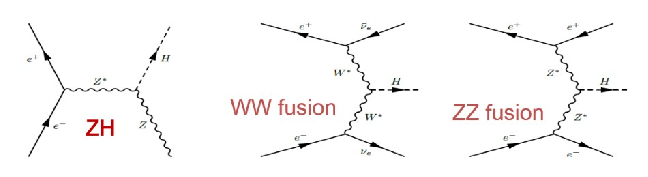
\includegraphics[width=0.75\textwidth]{FMD}
\caption[]{Feynman diagram of production of Higgs boson at CEPC}
\label{fig:fmd}
\end{center}
\end{figure}

%\subsection{Measurement of width of Higgs boson}
%In nonrelative quantum dynamics, the eigenvalue of hamitonian of free particle is mass. For a unstable particle, 
%its probability of existing in whole space is a function of time, $e^{-\Gamma t}$. $\Gamma$ in which is width. the physical 
%meaning is width of the function of mass's probability inducing to half of the highest.
%
%As we all known, the width of a particle is equal to sum of width product branch ratio of each decay mode. Once the width 
%has been measured, compared to the total width, we can know if the decay modes of this particle are complete. 
%
%Because the mass of Higgs boson is 125$\gev$, three decay modes, which have strong Yukawa coupling, $H\rightarrow t\bar{t}$, 
%$H\rightarrow WW$ and $H\rightarrow ZZ$, have been abstained. It makes width narrow enough, about 4$\mev$. Because the mass 
%resolution of LHC is 3 order higher than width of Higgs boson, the measurement of width is not very well in LHC. But we can 
%measure width indirectly through measurement of the absolute branch ratio of Higgs boson in CEPC. 
%
%To measure the width, we introduce four independent observables firstly:
%\begin{eqnarray}
%Y_1 = \sigma_{ZH} = F_1\cdot g_Z^2,
%\end{eqnarray}
%\begin{eqnarray}
%Y_2 = \sigma_{ZH} \cdot Br(H \rightarrow b\bar{b}) = F_2 \cdot \frac{g_Z^2g_b^2}{\Gamma_H},
%\end{eqnarray}
%\begin{eqnarray}
%Y_3 = \sigma_{\nu\bar{\nu}H} \cdot Br(H \rightarrow b\bar{b}) = F_3 \cdot \frac{g_W^2g_b^2}{\Gamma_H},
%\end{eqnarray}
%\begin{eqnarray}
%Y_4 = \sigma_{ZH} \cdot Br(H \rightarrow b\bar{b}) = F_4 \cdot \frac{g_W^2g_W^2}{\Gamma_H},
%\end{eqnarray}
%where $g_Z$, $g_W$ and $g_b$ are couplings of Higgs to $ZZ$,$ WW$ and $b\bar{b}$ respectively;
%$F_1$, $F_2$, $F_3$ and $F_4$ are factors which can be calculated unambiguously. With these
%four observable the couplings and total width can be obtained as follows:
%\begin{itemize}
%\item From the measurement of $Y_1$ we can get the coupling $g_Z = \sqrt{\frac{Y_1}{F_1}}$,
%\item From the ratio $Y_2/Y_3$ we can get the coupling ratio $g_Z/g_W = \sqrt{\frac{Y_2F_3}{Y_3F_2}}$,
%\item With $g_Z$ and $g_Z/g_W$, we can get $g_W = \sqrt{\frac{Y_1Y_3F_2}{Y_2F_1F_3}}$,
%\item With $g_Z$ and $g_W$ known, from the measurement of $Y_4$ we can get the Higgs
%total width $\Gamma_H = \frac{Y_1^2Y_3F_2F_4}{Y_2Y_4F_1^2F_3}$.
%\end{itemize}
%In this note, we can get a important input for measurement, the branch ratio of $H\rightarrow WW^*$. And the other results 
%would be given by other collabration or CEPC.

\subsection{Class of signal processs}
The full simulation study of Br($H\rightarrow WW^*$) measurements at the CEPC has strong physics initersts. First of all, 
the nominal SM Higgs boson has 22\% chance to decay into a pair of $W$ boson, therefore this measurement is the most substantial channel 
to study Higgs to vector boson coupling behaviors at the CEPC. Secondly, the Br($H\rightarrow WW^*$) measurement is also 
a key ingredient for the determination of Higgs boson width. Last but not least, the $W$ boson decays into various physics 
objects(leptons, missing energy and momentum, taus and jets), therefore it provides an excellent benchmark for the detector 
performance studies. A series of Br($H\rightarrow WW^*$) full simulation study has been performed and  
status of these studies would be reported in this manuscript. 

The $H\rightarrow WW^*$ events at the CEPC could be classified into 50 different channels according to final 
states of events. Giving one million Higgs bosons, the expected yield for $H\rightarrow WW^*$ events with different 
final states are presented in Table~\ref{tab:list}. Our simulation studies has covered the following channels, which is 
classified into 4 kinds according to the number of jets in the final states.
\begin{table}[H]
  \begin{center}
    \begin{tabular}{|c|c|c|c|c|c|}
      \hline \hline
      \backslashbox{$W$ boson decay}{$Z$ boson decay}      & $ee$ & $\mu\mu$ & $\tau\tau$ & $\nu\nu$ & $qq$ \\
      \hline
      $WW^*\rightarrow e\nu e\nu$	&	\multicolumn{1}{>{\columncolor{mygray}}c|}{95}	
	  								&	\multicolumn{1}{>{\columncolor{mygray}}c|}{89}	
									&	\multicolumn{1}{>{\columncolor{mygray}}c|}{89} 	
									&	\multicolumn{1}{>{\columncolor{mygray}}c|}{612} 	
									&	\multicolumn{1}{>{\columncolor{green}}c|}{1791}\\
	  \hline                                                                
      $WW^*\rightarrow \mu\nu\mu\nu$&	\multicolumn{1}{>{\columncolor{mygray}}c|}{94}	
	  								&	\multicolumn{1}{>{\columncolor{mygray}}c|}{87}	
									&	\multicolumn{1}{>{\columncolor{mygray}}c|}{87}	
									&	\multicolumn{1}{>{\columncolor{mygray}}c|}{601}		
									&	\multicolumn{1}{>{\columncolor{green}}c|}{1758}\\
      \hline                                                                
      $WW^*\rightarrow e\nu\mu\nu$	&	\multicolumn{1}{>{\columncolor{mygray}}c|}{188}	
	  								&	\multicolumn{1}{>{\columncolor{mygray}}c|}{176}	
									&	\multicolumn{1}{>{\columncolor{mygray}}c|}{176}	
									&	\multicolumn{1}{>{\columncolor{mygray}}c|}{1212}	
									&	\multicolumn{1}{>{\columncolor{green}}c|}{3548}\\
      \hline                                                                
	  $WW^*\rightarrow e\nu\tau\nu$	&	\multicolumn{1}{>{\columncolor{mygray}}c|}{201}	
	  								&	\multicolumn{1}{>{\columncolor{mygray}}c|}{188}	
									&	\multicolumn{1}{>{\columncolor{mygray}}c|}{187}	
									&	\multicolumn{1}{>{\columncolor{mygray}}c|}{1292}	
									&	\multicolumn{1}{>{\columncolor{green}}c|}{3783}\\
	  \hline                                                                
	  $WW^*\rightarrow \mu\nu\tau\nu$&	\multicolumn{1}{>{\columncolor{mygray}}c|}{109}	
	  								&	\multicolumn{1}{>{\columncolor{mygray}}c|}{186}	
									&	\multicolumn{1}{>{\columncolor{mygray}}c|}{186}	
									&	\multicolumn{1}{>{\columncolor{mygray}}c|}{1280}	
									&	\multicolumn{1}{>{\columncolor{green}}c|}{3747}\\
	  \hline                                                                
	  $WW^*\rightarrow \tau\nu\tau\nu$&	\multicolumn{1}{>{\columncolor{mygray}}c|}{156}	
	  								&	\multicolumn{1}{>{\columncolor{mygray}}c|}{99}	
									&	\multicolumn{1}{>{\columncolor{mygray}}c|}{99}	
									&	\multicolumn{1}{>{\columncolor{mygray}}c|}{683}		
									&	\multicolumn{1}{>{\columncolor{green}}c|}{1998}\\
      \hline                                                                
      $WW^*\rightarrow e\nu qq$		&	\multicolumn{1}{>{\columncolor{green}}c|}{1195}
	  								&	\multicolumn{1}{>{\columncolor{green}}c|}{1117}
									&	\multicolumn{1}{>{\columncolor{green}}c|}{1115}
									&	\multicolumn{1}{>{\columncolor{green}}c|}{7704}	
									&	\multicolumn{1}{>{\columncolor{magenta}}c|}{22560}\\
      \hline                                                                
      $WW^*\rightarrow \mu\nu qq$ 	&	\multicolumn{1}{>{\columncolor{green}}c|}{1184}
	  								&	\multicolumn{1}{>{\columncolor{green}}c|}{1106}
									&	\multicolumn{1}{>{\columncolor{green}}c|}{1104}
									&	\multicolumn{1}{>{\columncolor{green}}c|}{7632}	
									&	\multicolumn{1}{>{\columncolor{magenta}}c|}{22349}\\
      \hline                                                                
	  $WW^*\rightarrow \tau\nu qq$	&	\multicolumn{1}{>{\columncolor{green}}c|}{1263}
	  								&	\multicolumn{1}{>{\columncolor{green}}c|}{1180}
									&	\multicolumn{1}{>{\columncolor{green}}c|}{1177}
									&	\multicolumn{1}{>{\columncolor{green}}c|}{8136}	
									&	\multicolumn{1}{>{\columncolor{magenta}}c|}{23825}\\
	  \hline                                                                
	  $WW^*\rightarrow qqqq$ 		&	\multicolumn{1}{>{\columncolor{magenta}}c|}{3764}
	  								&	\multicolumn{1}{>{\columncolor{magenta}}c|}{3518}
									&	\multicolumn{1}{>{\columncolor{magenta}}c|}{3510}
									&	\multicolumn{1}{>{\columncolor{magenta}}c|}{24264}	
									&	\multicolumn{1}{>{\columncolor{red}}c|}{71051}\\
      \hline \hline
    \end{tabular}
   \caption[Monte Carlo purities in the single lepton sample]{Excepted signal events of $Z\rightarrow X, H\rightarrow WW^*, 
	   WW^* \rightarrow X$.  
   The gray area means there are no jets in signal events. 
   The green district represents the class of two jets. The four jets events are indicated by magenta.
   And the red one repersents six jets events.}
  \label{tab:list}
 \end{center}
\end{table}

In this note, a representative analysis of each kind is reported in detail. For type of zero jet, 
$e^+e^-\rightarrow ZH, Z\rightarrow \mu^+\mu^-,  H\rightarrow WW^*, WW^*\rightarrow e\nu\mu\nu$ decay channel has been 
choosed. 
$e^+e^-\rightarrow ZH, Z\rightarrow e^+e^-,  H\rightarrow WW^*, WW^*\rightarrow \mu\nu qq$ decay channel is a candidate for 
type of two jets. And for four jets events, $e^+e^-\rightarrow ZH, Z\rightarrow \nu\nu,  H\rightarrow WW^*, WW^*\rightarrow qqqq$ 
decay channel has been choosed as the typical channel. The unique channel for six jets is complicated and would be analyzed in the future.

%This manuscript is organized as following. The second section described the detector geometry implemented in the full simulation. 
%The MC sample,simulation and reconstruction tools are introduced, and to reduce the consumption of computing power, general 
%event filters has been applied to the CEPC Higgs analsis, which is reported in section 3. Section 4 is devided into three parts, 
%each corresponding to one representative analysis of different $H\rightarrow WW^*$ decay mode. In section 5, the results of all 
%individual analysis are combined, leading to an accuracy of Br($H\rightarrow WW^*$) measurement. Conclusion and outlooks are 
%summarized in Section 6.

%\section{The CEPC detector}
%The CEPC conceptual detector design is based on ILC detector designs, as illustrated in Figure~\ref{fig:acepcdetector}. 
%\begin{figure}[H]
%	\centering
%	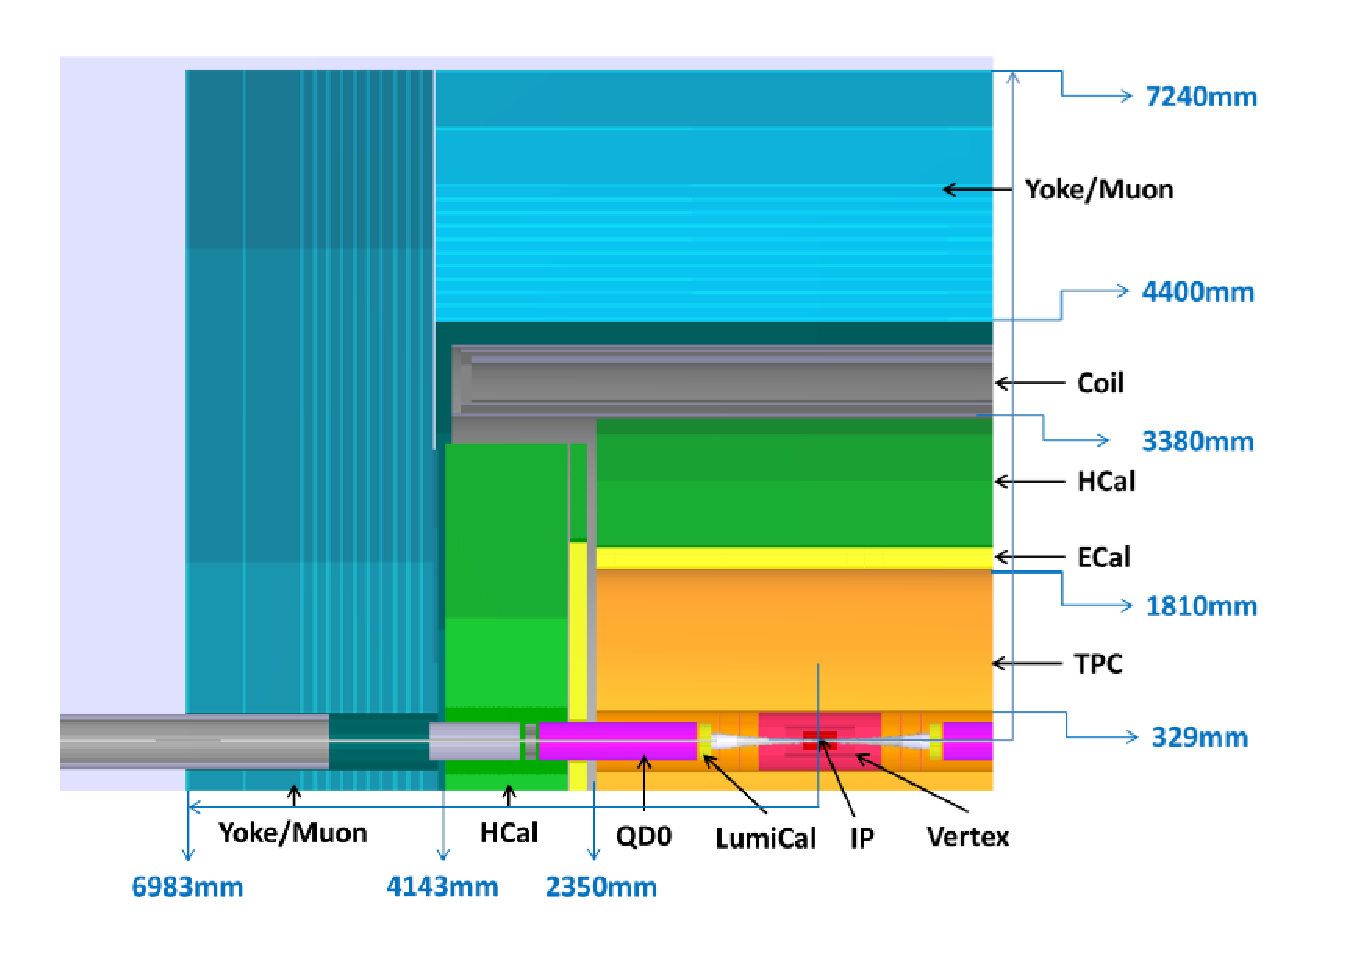
\includegraphics[width=0.7\textwidth]{cepcdetector}
%	\caption[]{Overview of the CEPC detector}
%	\label{fig:acepcdetector}
%\end{figure}
%The CEPC detectoe consists of the following sub-detectors:
%\begin{itemize}
%	\item A vertex detector(VTX) construted with high resolution pixel sensors. 
%		The vertex detector is placed very close to the intreaction point, withan inner radius of 16mm. 
%		This vertex detector ensures excellent tagging capability of $b\text{-}/c\text{-}$quark jets and $\tau\text{-}$leptons.
%	\item A silicon tracker composed of Silicon Inner Tracker(SIT), Forward Tracking Disks(FTDs), 
%		Silicon External Tracker(SET) and End-cap Tracking Disks(ETDs). The VTX and SIT provide 
%		excellent spatial measurement near the IP, crucial for vertex reconstruction and jet flavor tagging. 
%		The SET and ETD, on the other handm provide excellent spatial resolution with the maximal possible 
%		track arm length, therefore improving the track momentum resolution of charged particles. 
%		The FTDs significantly increases the geometric acceptance of the tracking system with coverage of $|\cos\theta| < 0.99$. 
%	\item A Time Projection Chanber(TPC) with a half-length of 2.35m and an outer radius of 1.8m.
%		The TPC provides a large number of spatial points ($\sim$200 hits per track) and spatial resolution 
%		in $r\phi$ plane better than 100$\mu$m. It has excellent pattern recognition and track reconstruction 
%		efficiency(better than 97\% for tracks with $p_T > 1\gev$).
%	\item A calorimetry system consists of Electromagnetic Calorimeter(ECal) and Hadron Calorimeter(HCal) 
%		with very fine granularity. The system plays an essential role in the Particle-Flow Algorithm(PFA), 
%		allowing excellent separation of showers from different particles, and provides jet energy resolution of 3 - 4\%.
%	\item A superconducting solenoid of 3.5T surrounds the calorimetry system. The return yoke is placed outside the solensid. 
%	\item A muon detector with tracking layers installed in the return yoke. 
%\end{itemize}

\section{MC sample}
\subsection{Simulation and analysis tool}
This analysis is performed with a simulated data of integrated luminosity of 5000fb$^{-1}$, and the cross section at $\sqrt s =250\gev$
is shown in Figure~\ref{fig:cs}. 
For all signal, which Higgs mass of $m_H = 125\gev$ is assumed, and background events are generated by Whizard 1.95 included ISR. 
The detector model, cepc\_v1, is simulated by Gent4. Particle reconstruction is done by particle-flow algorithm, Arbor. 
Charged particle idendifications are done by LICH, which is a TMVA based charged particle identification using high graularity calorimeter. 
The $ee$-$k_T$ clustering algorithm is used in jet clustering and the $b$-tagging probabilities is given by LCFIPlus package.

\begin{figure}[H]
	\centering
	\subfigure[]{
		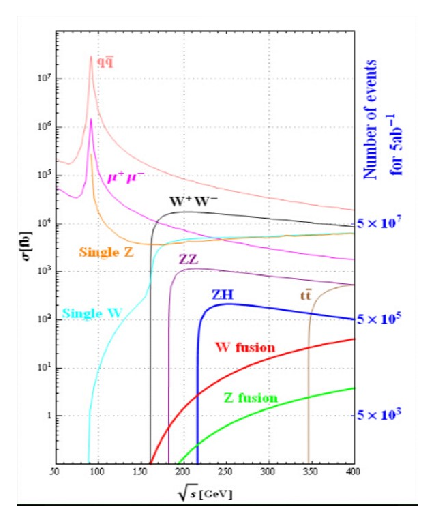
\includegraphics[width=0.35\textwidth]{CSF}
		\label{fig:csf}
	}
	\subfigure[]{
		 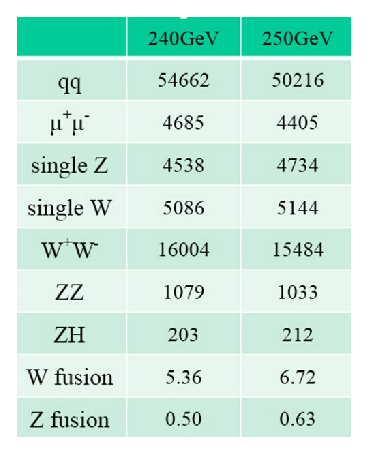
\includegraphics[width=0.35\textwidth]{CST}
		 \label{fig:cst}
	}
	\caption[]{\ref{fig:csf}: The distribution of cross sction of the Standard Model when center mass of system is near $250\gev$.
	\ref{fig:cst}: The specific value of cross section of the main Standard Model when center mass of system is $240\gev$ and $250\gev$}
	\label{fig:cs}
\end{figure}

The Standard Model background contain two femions background and four femions background.
Two femions background include processes of bhabha scatter, $\mu^+\mu^-$, $\tau^+\tau^-$, $\nu\bar{\nu}$ and $q\bar{q}$.
Four femions background consist of rest of the Standard Model background and Higgs Background.
Higgs background is the $ZH$ process except for the signal process.

\subsection{Pre-selection}
After counting the total background, the number of the Standard Model is more than 70 million.
However, because of lack of computer resource, the SM background is simulated and reconstructed only a part, 
and many events of them have completely different event topology comparing to signal events, 
especially after signal catelogy according to the flavor of adjoint fermions. 
According to the event topology, the Higgs signals are cataloged into 4 classes, $llH(l=e,\mu)$, $\tau\tau H$, 
$\nu\nu H$ and $qqH$. 

Therefore, the Standard Model background would be selected at truth level before simulation and reconstruction 
based on the different kinds of signal events. To make the pre-selection more consistency, reasonable and available 
in reconstruction level, every conditions of pre-selection should be loose at MC level, to preserve the signal almostly. 

\subsubsection{Pre-selection of $e^+e^- \rightarrow ZH, Z\rightarrow l^+l^-(l=e,\mu), H\rightarrow X$ decay}
Compared to the Standard Model background, the most remarkable feature in $Z\rightarrow l^+l^-(l=e,\mu), H\rightarrow X$ 
decay channel is the combination of invariant mass and recoil mass of $Z$ boson. 
Just like the real situation in detector, the best candidate of $Z$ boson by consisted of leptons should be found. 
As shown in Table~\ref{tab:llhprecut}, here are two conditions of filter. Fisrt one is invariant mass of $l^+l^-$.
The second is corresponding recoil mass. %And the plots of invariant mass and recoil mass are in Appendix~\ref{}. 
\begin{figure}[H]
	\centering
	\subfigure[]{
		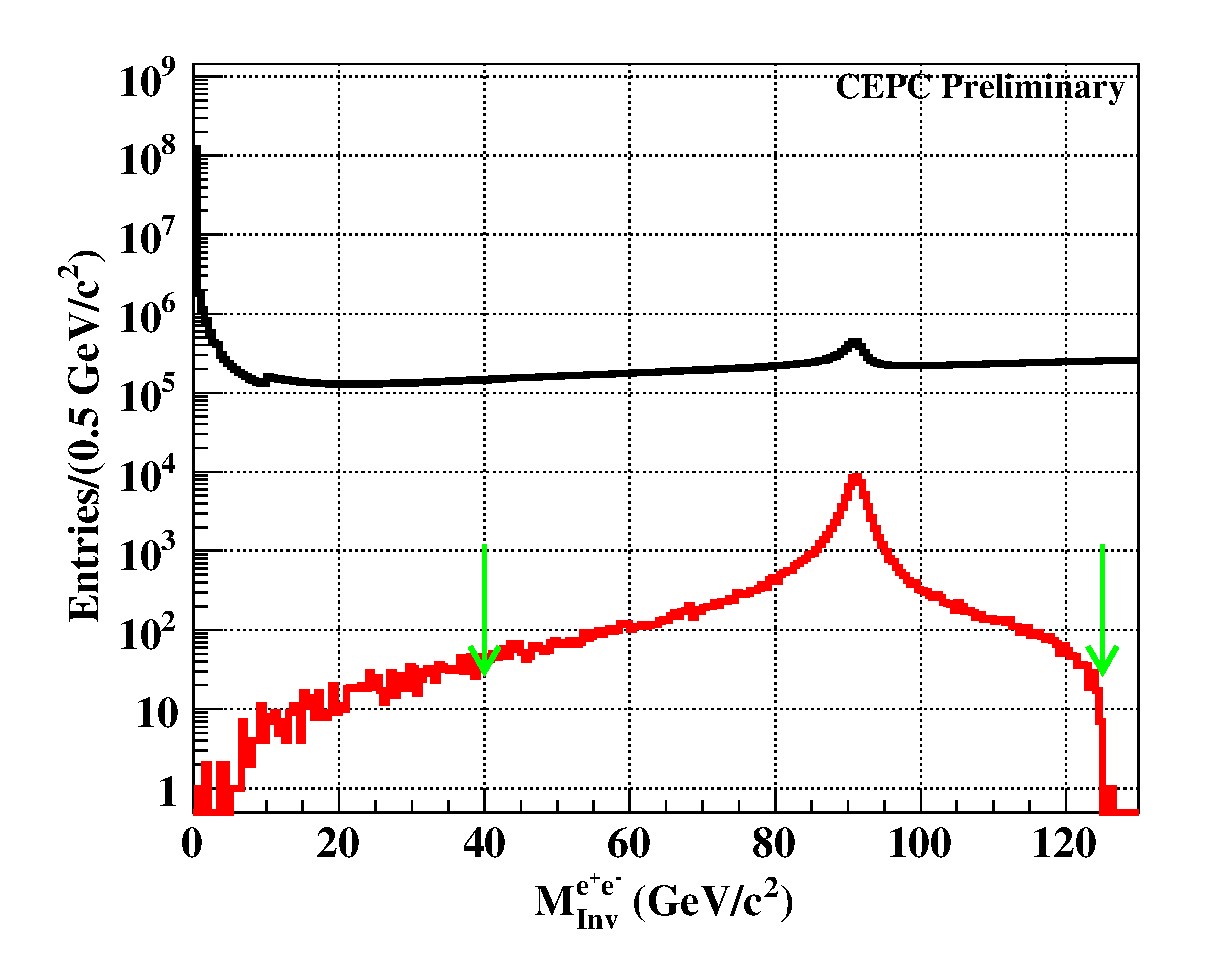
\includegraphics[width=0.35\textwidth]{filterfig/mcfig/e1e1H/eeHInvMass}
		\label{fig:eeHfilterInvMass}
	}
	\subfigure[]{
		 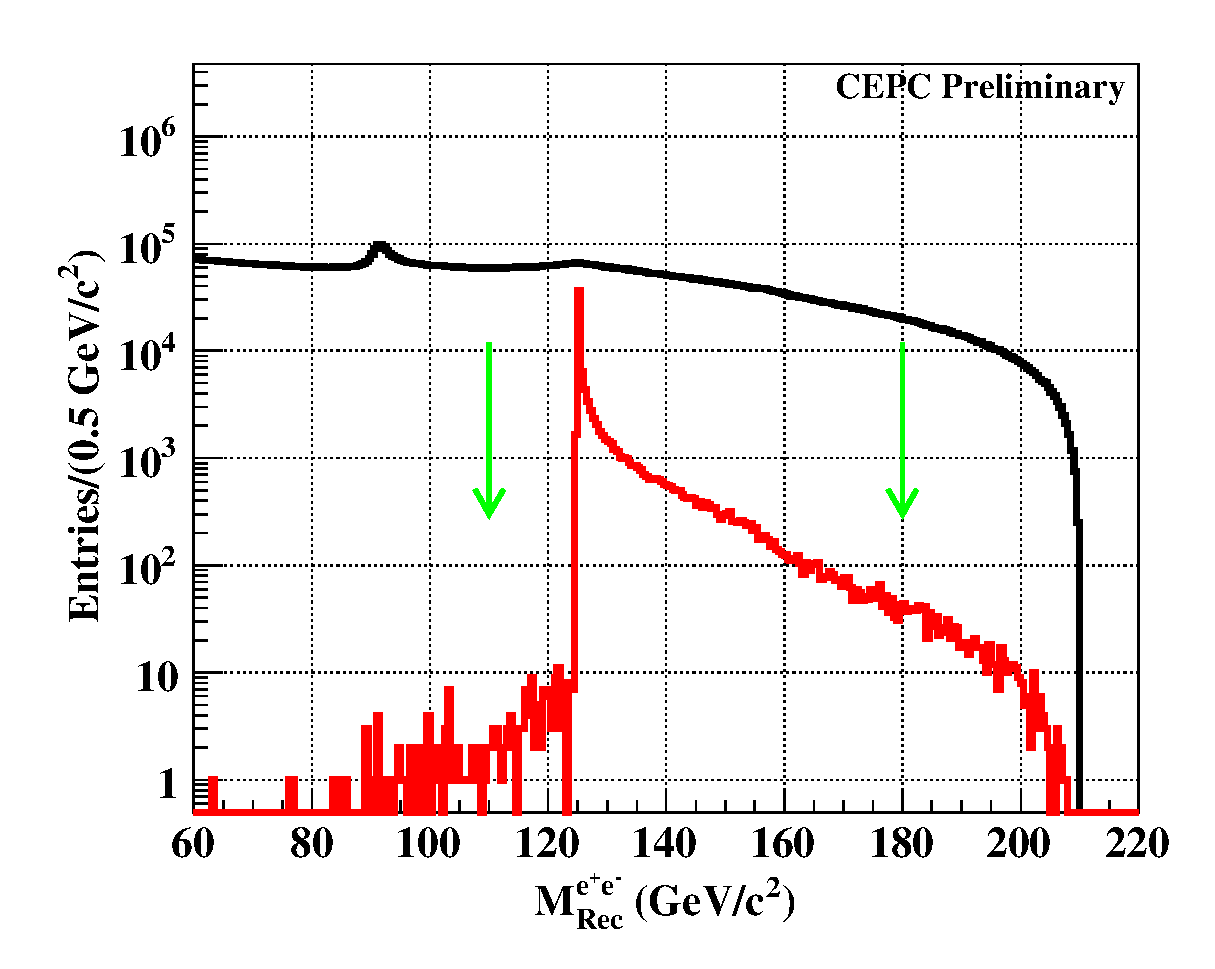
\includegraphics[width=0.35\textwidth]{filterfig/mcfig/e1e1H/eeHRecMass}
		 \label{fig:eeHfilterRecMass}
	}
	\subfigure[]{
		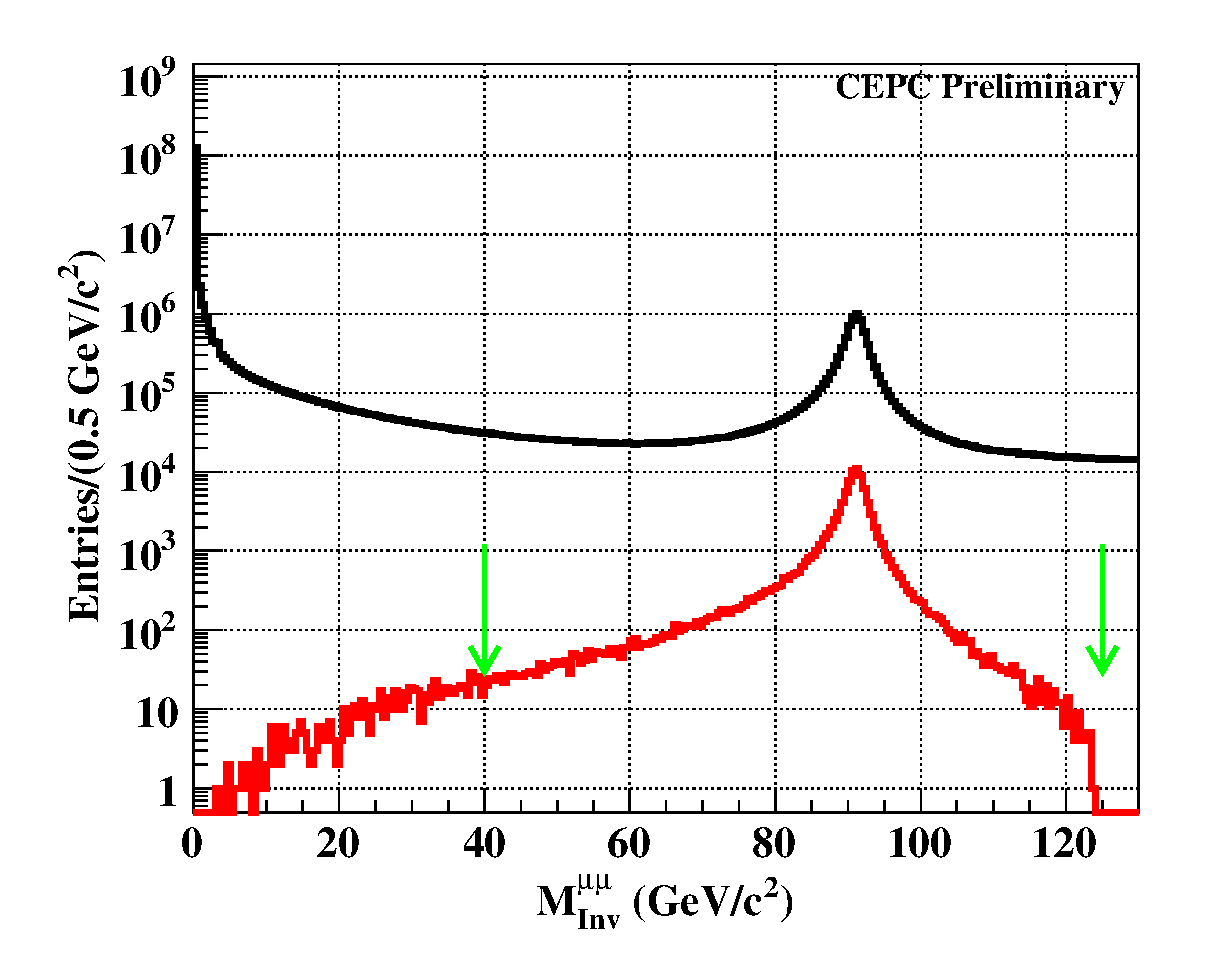
\includegraphics[width=0.35\textwidth]{filterfig/mcfig/e2e2H/uuHInvMass}
		\label{fig:uuHfilterInvMass}
	}
	\subfigure[]{
		 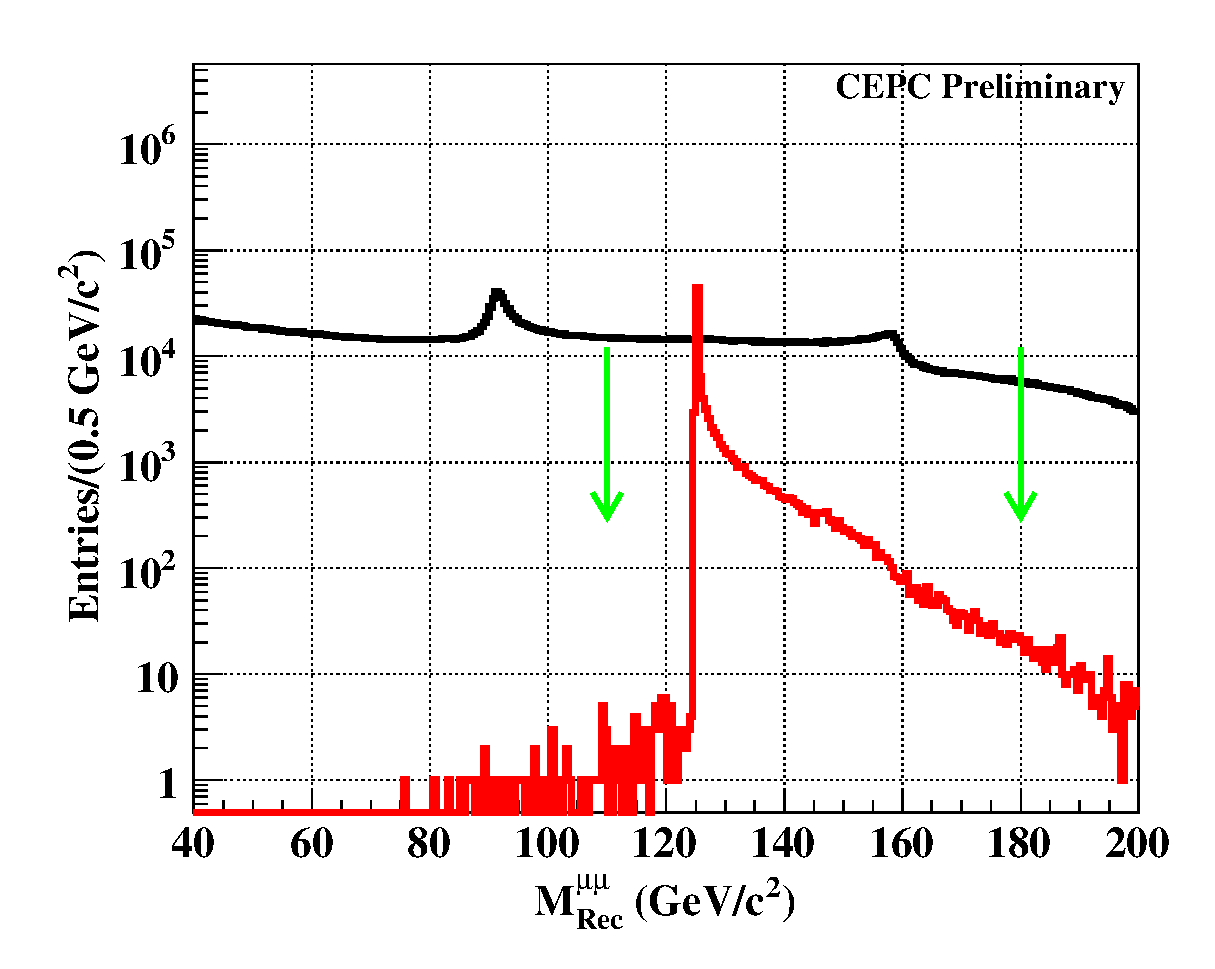
\includegraphics[width=0.35\textwidth]{filterfig/mcfig/e2e2H/uuHRecMass}
		 \label{fig:uuHfilterRecMass}
	}
	\caption[]{The distribution of invariant mass and recoil mass of the best candidate of $Z$ boson. 
	Red line is the distribution of Higgs signal. Black line is the distribution of the Standard Model background.
	TOP: These two plots are the mass distribution of $Z\rightarrow e^+e^-, H\rightarrow X$ decay.
	Bottom: The left is invariant mass distribution and right is recoil mass distribution of $Z\rightarrow \mu^+\mu^-, H\rightarrow X$ decay}
	\label{fig:llHfilter}
\end{figure}
\begin{figure}[H]
	\centering
	\subfigure[]{
		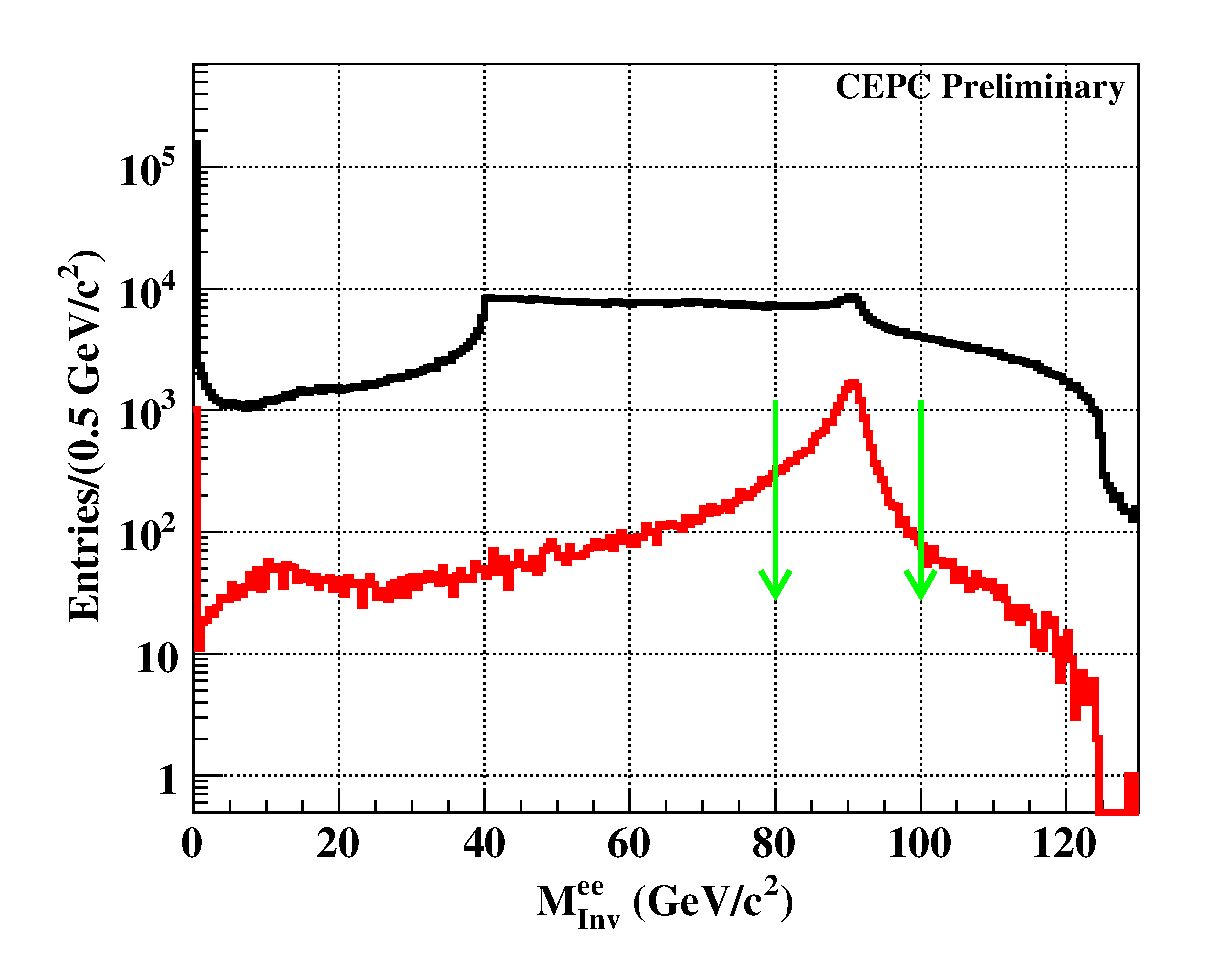
\includegraphics[width=0.35\textwidth]{filterfig/fullsim/e1e1H/InvMass}
		\label{fig:eeHfilteredInvMass}
	}
	\subfigure[]{
		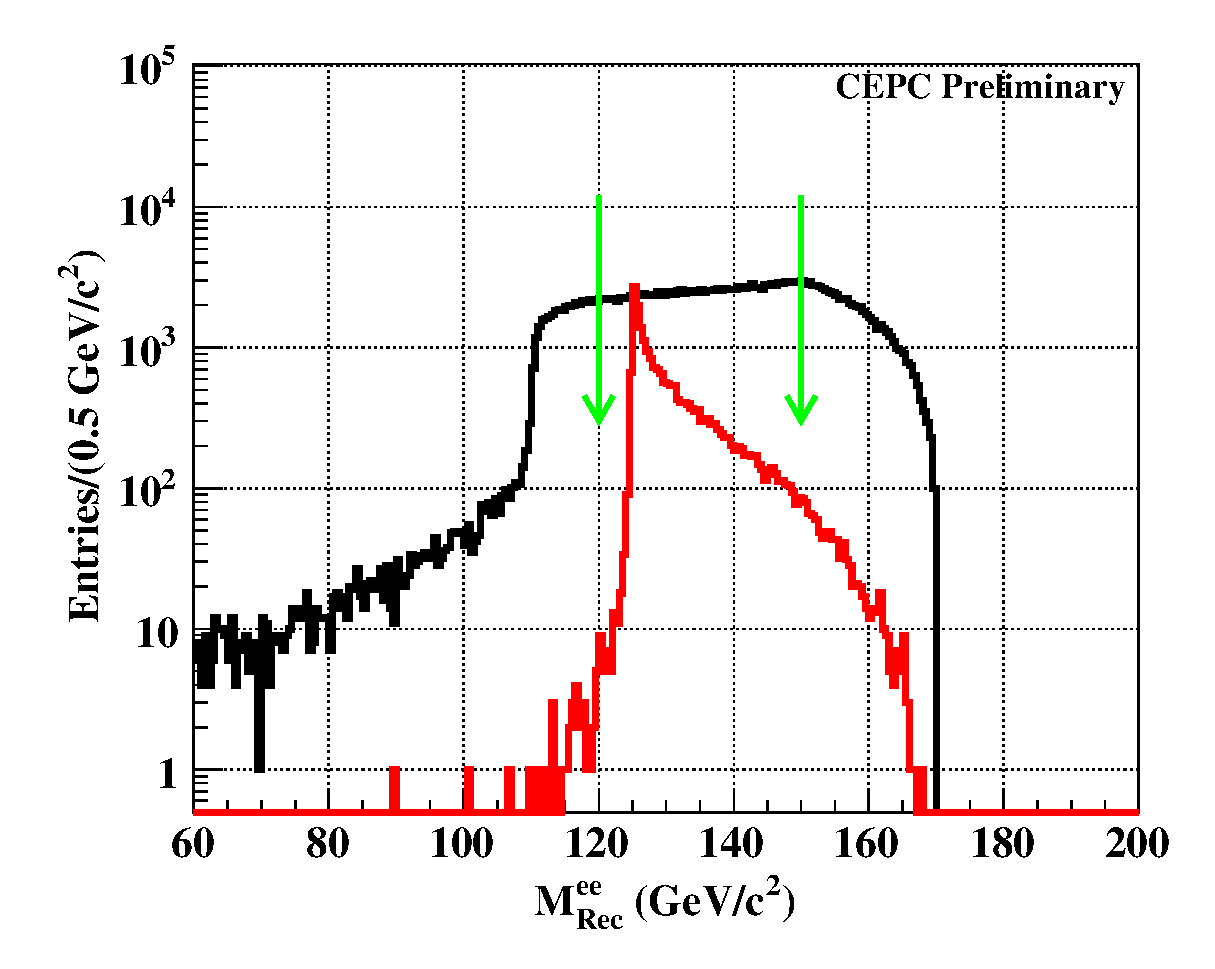
\includegraphics[width=0.35\textwidth]{filterfig/fullsim/e1e1H/RecMass}
		\label{fig:eeHfilteredRecMass}
	}
	\subfigure[]{
		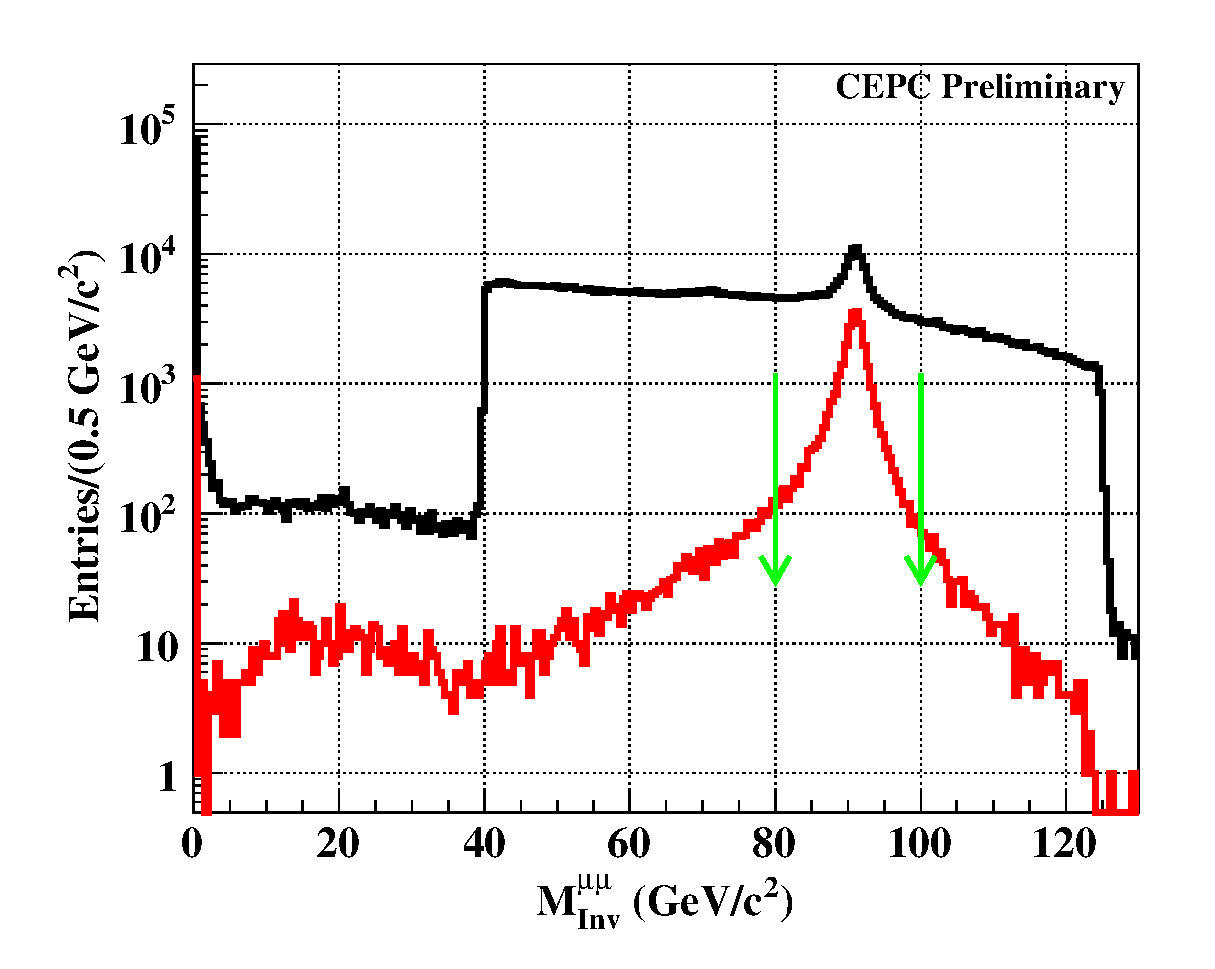
\includegraphics[width=0.35\textwidth]{filterfig/fullsim/e2e2H/InvMass}
		\label{fig:uuHfilteredInvMass}
	}
	\subfigure[]{
		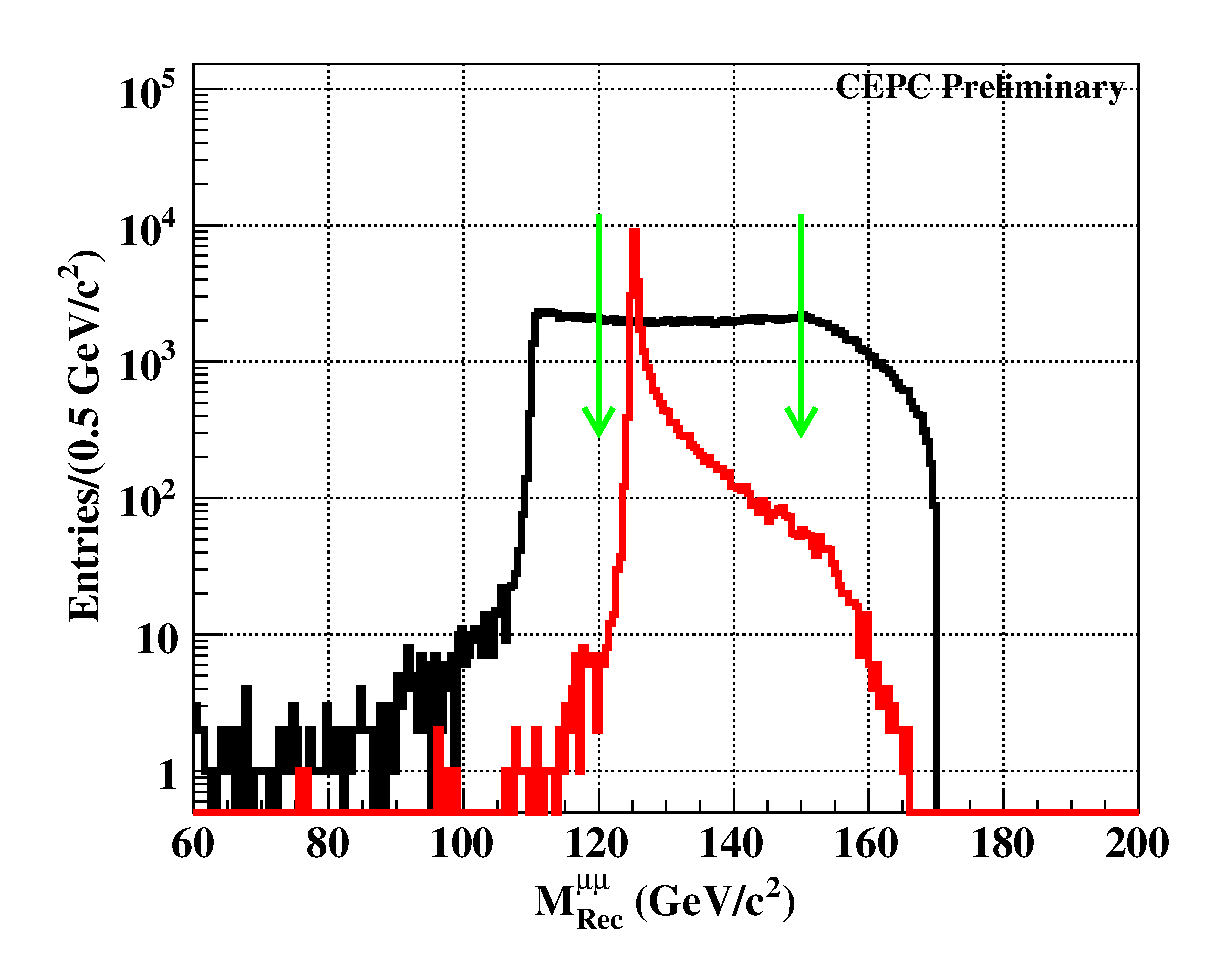
\includegraphics[width=0.35\textwidth]{filterfig/fullsim/e2e2H/RecMass}
		\label{fig:uuHfilteredRecMass}
	}
	\caption[]{The distribution of invariant mass and recoil mass of the best candidate of $Z$ boson in full simulation. 
	Red line is the distribution of Higgs signal. Black line is the distribution of the Standard Model background.
	TOP: These two plots are the mass distribution of $Z\rightarrow e^+e^-, H\rightarrow X$ decay.
	Bottom: The left is invariant mass distribution and right is recoil mass distribution of $Z\rightarrow \mu^+\mu^-, H\rightarrow X$ decay}
	\label{fig:llHfiltered}
\end{figure}

\begin{table}[H]
\newcommand{\tabincell}[2]{\begin{tabular}{@{}#1@{}}#2\end{tabular}}
 \begin{center}
  \begin{tabular}{|c|c|c|}
  \hline \hline
  Process of signal				&		$eeH$ process						&				$\mu\mu H$ process\\
  \hline
  \multirow{2}{*}{conditions of pre-selection} 	&	$40\gev/c^2 < M_{Inv}^{ee} < 130\gev/c^2$&$40\gev/c^2 < M_{Inv}^{\mu\mu} < 130\gev/c^2$	\\
  											&	$110\gev/c^2 < M_{Rec}^{ee} < 180\gev/c^2$		&$110\gev/c^2 < M_{Rec}^{\mu\mu} < 180\gev/c^2$\\
  \hline
  \multirow{2}{*}{conditions of validation}	&	$80\gev/c^2 < M_{Inv}^{ee} < 100\gev/c^2$&$80\gev/c^2 < M_{Inv}^{\mu\mu} < 100\gev/c^2$	\\
  											&	$120\gev/c^2 < M_{Rec}^{ee} < 150\gev/c^2$		&$120\gev/c^2 < M_{Rec}^{\mu\mu} < 150\gev/c^2$\\
  \hline \hline
  \end{tabular}
  \caption[]{Conditions of pre-selection in MC and validation in full simulation. Considered the resolution of detector, the conditions of 
  validation should be more strict.}
  \label{tab:llhprecut}
 \end{center}
\end{table}
After pre-selection, signal events have been preserved more than 95\% and background events have been rejected more than 99\% in truth. 
And there are no bias after pre-selection.

\subsubsection{Pre-selection of $e^+e^- \rightarrow ZH, Z\rightarrow \nu\bar{\nu}, H\rightarrow X$ decay.}
Compared to $eeH$ and $\mu\mu H$ processes. conditions of pre-selection of $\nu\nu H$ process are more difficult to choose. 
Because the $Z$ boson in $ZH$ process is decay to neutrino which is invisible in detector, it's hard to utilize the missing mass 
of system to distinguish signal and background clearly. For rejecting background extremely, we chose these three conditions: missing 
mass, total mass and total transvers momentum. In addtion, if $|cos\theta|$ of particle is larger than 0.99, 
it would be regard as missing particle.
\begin{figure}[H]
	\centering
	\subfigure[]{
		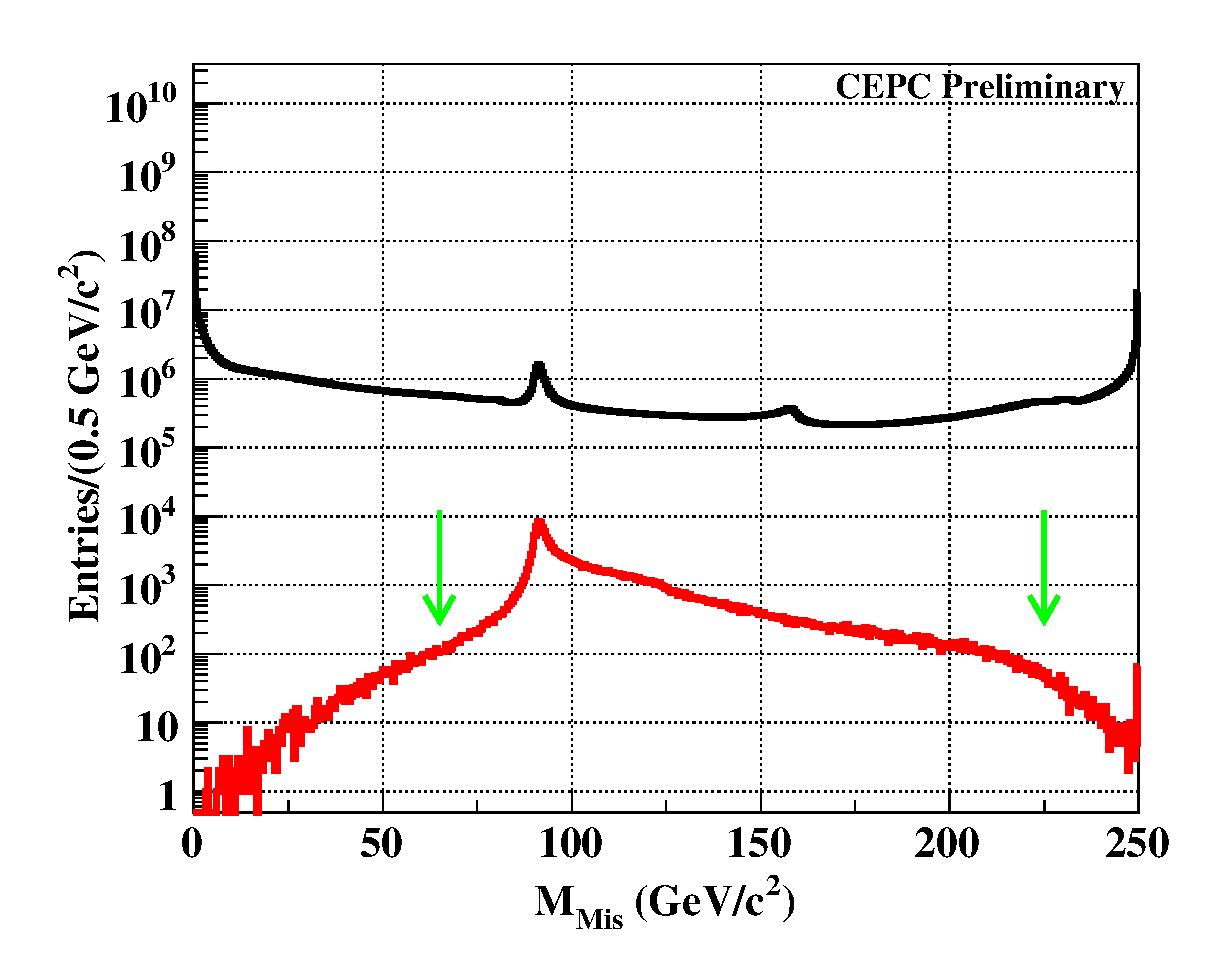
\includegraphics[width=0.35\textwidth]{filterfig/mcfig/nnH/MisMass}
		\label{fig:eeHfilterRecMass}
	}
	\subfigure[]{
		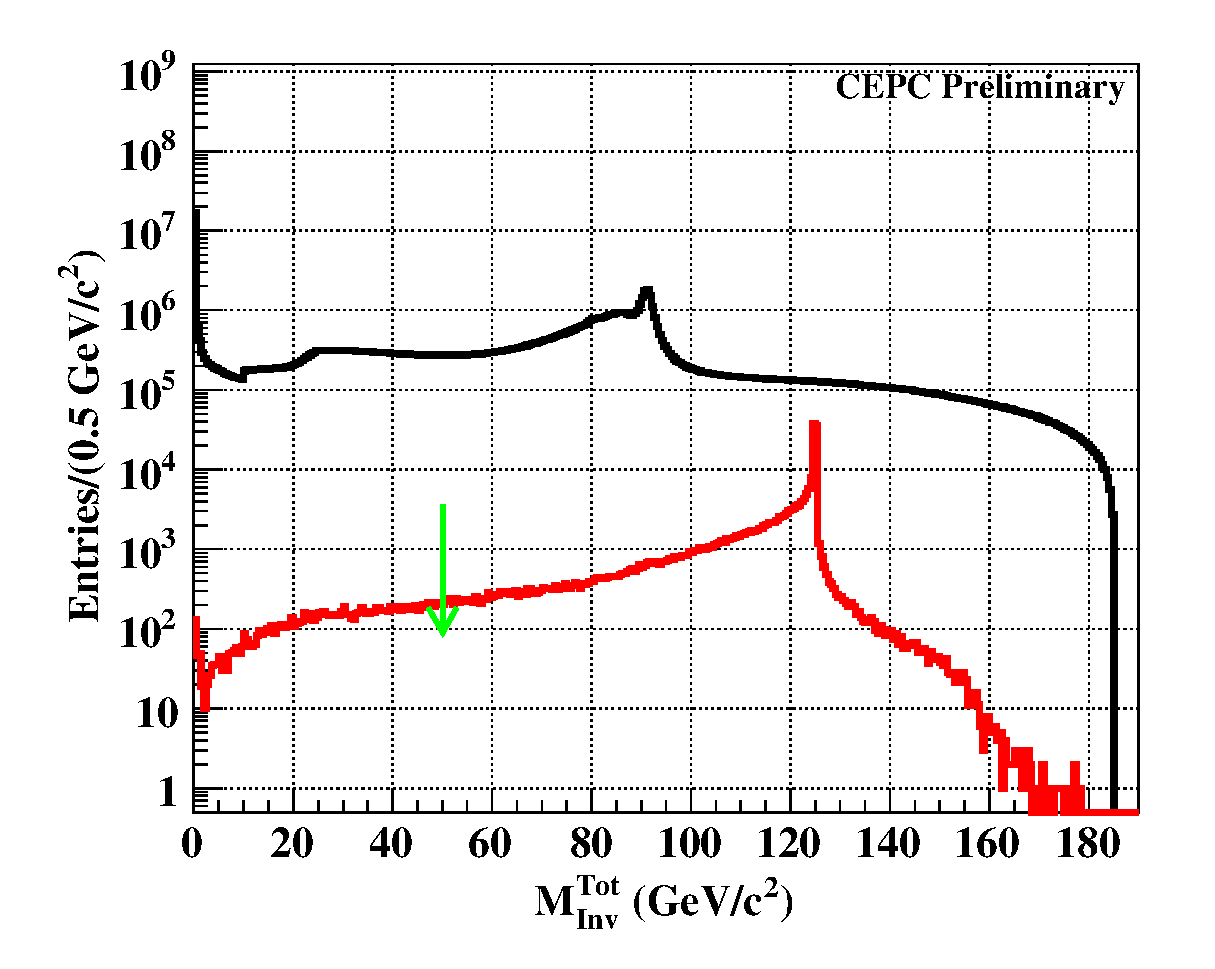
\includegraphics[width=0.35\textwidth]{filterfig/mcfig/nnH/TotalM}
		\label{fig:uuHfilterInvMass}
	}
	\subfigure[]{
		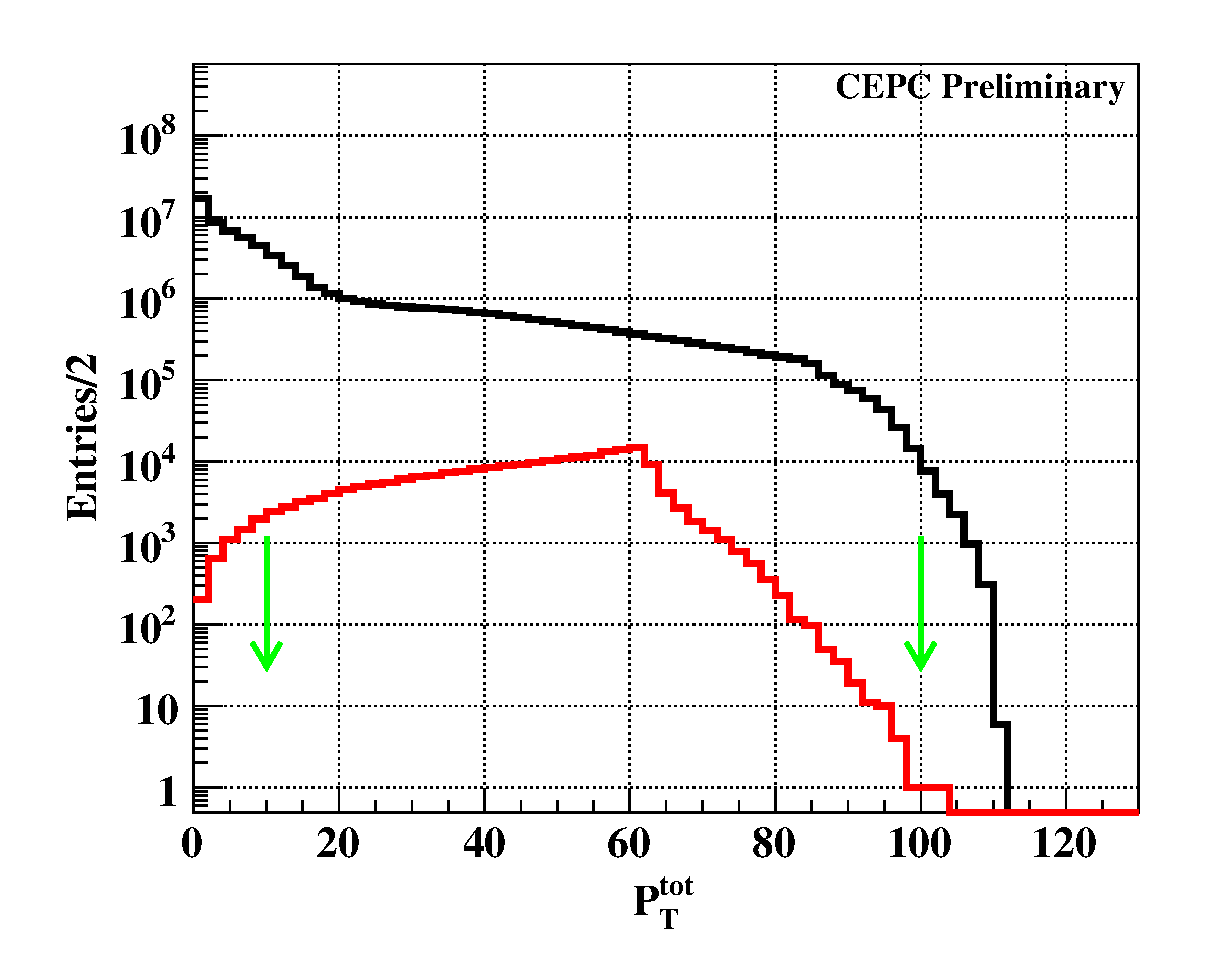
\includegraphics[width=0.35\textwidth]{filterfig/mcfig/nnH/TotalPt}
		\label{fig:uuHfiltedRecMass}
	}
	\caption[]{The distribution of missing mass, total mass and total transverse momentum in MC truth. 
	Red line is the distribution of Higgs signal. Black line is the distribution of the Standard Model background.
	Top: The left is missing mass of system. The right is total mass of system.
	Bottom: It is the distribution of total transverse momentum of system, and the peak of background is caused by angle constraint of 
	two femion background.}
	\label{fig:nnHfilter}
\end{figure}
\begin{figure}[H]
	\centering
	\subfigure[]{
		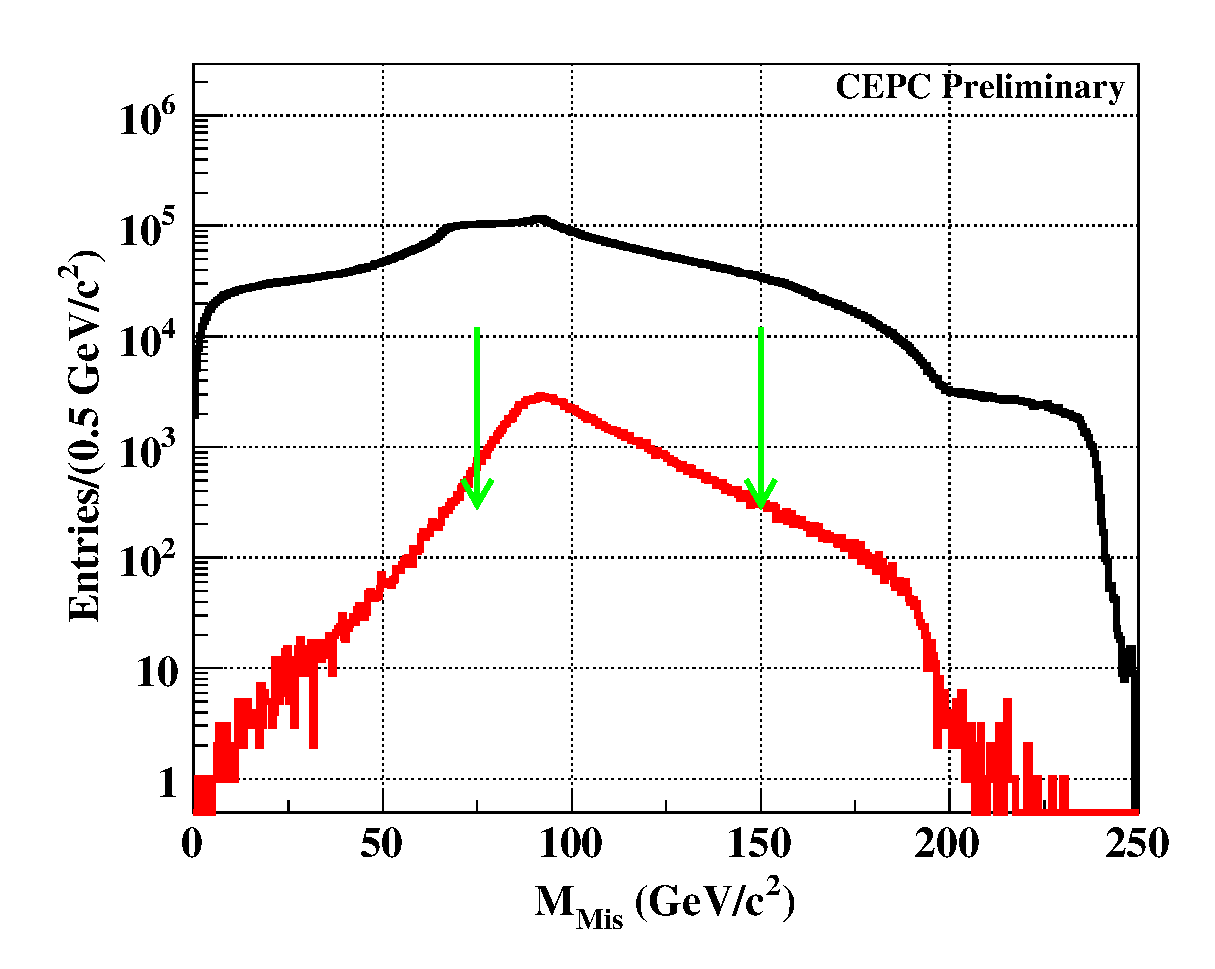
\includegraphics[width=0.35\textwidth]{filterfig/fullsim/nnH/MisMass}
		\label{fig:eeHfilteredRecMass}
	}
	\subfigure[]{
		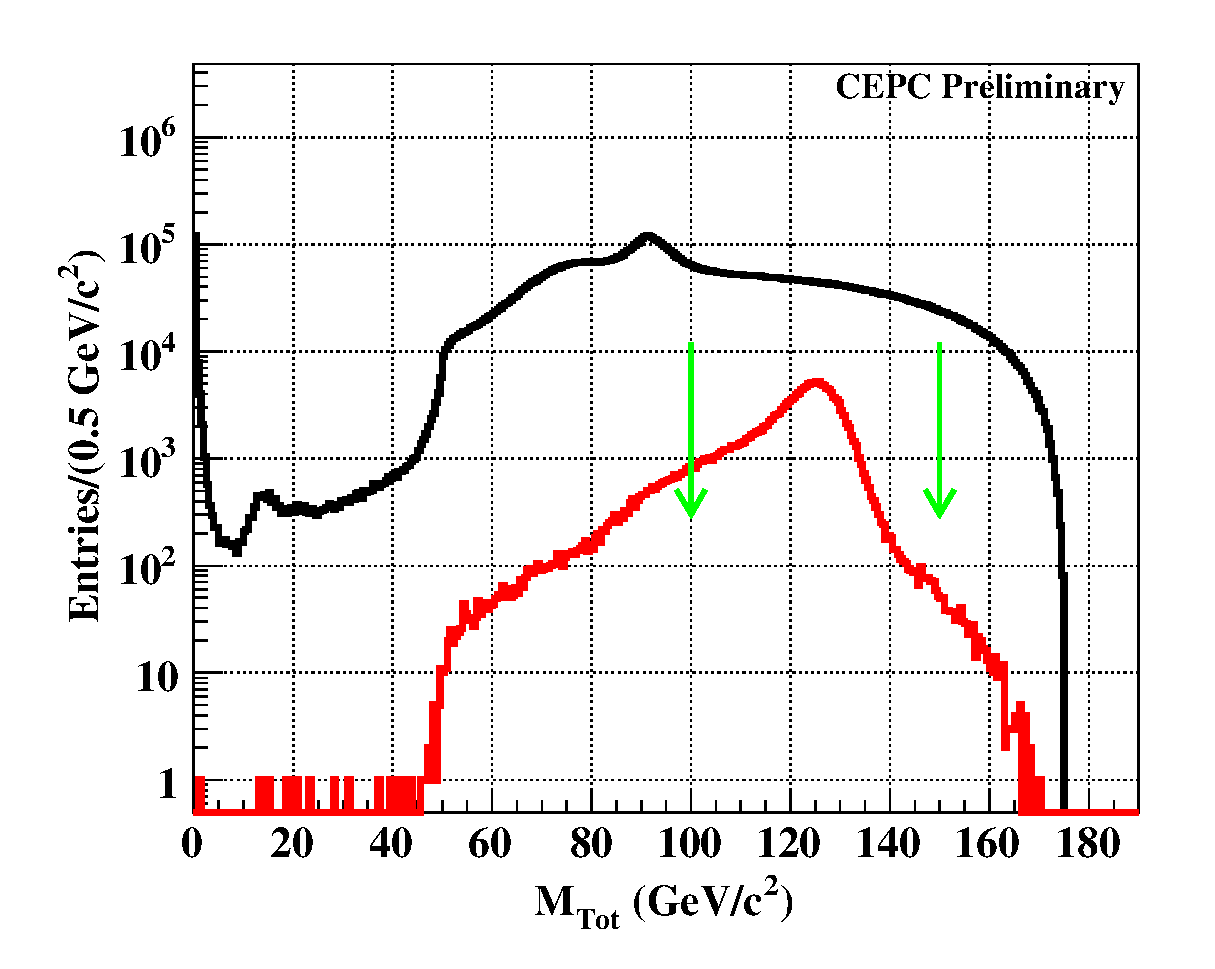
\includegraphics[width=0.35\textwidth]{filterfig/fullsim/nnH/TotalMass}
		\label{fig:uuHfilteredInvMass}
	}
	\subfigure[]{
		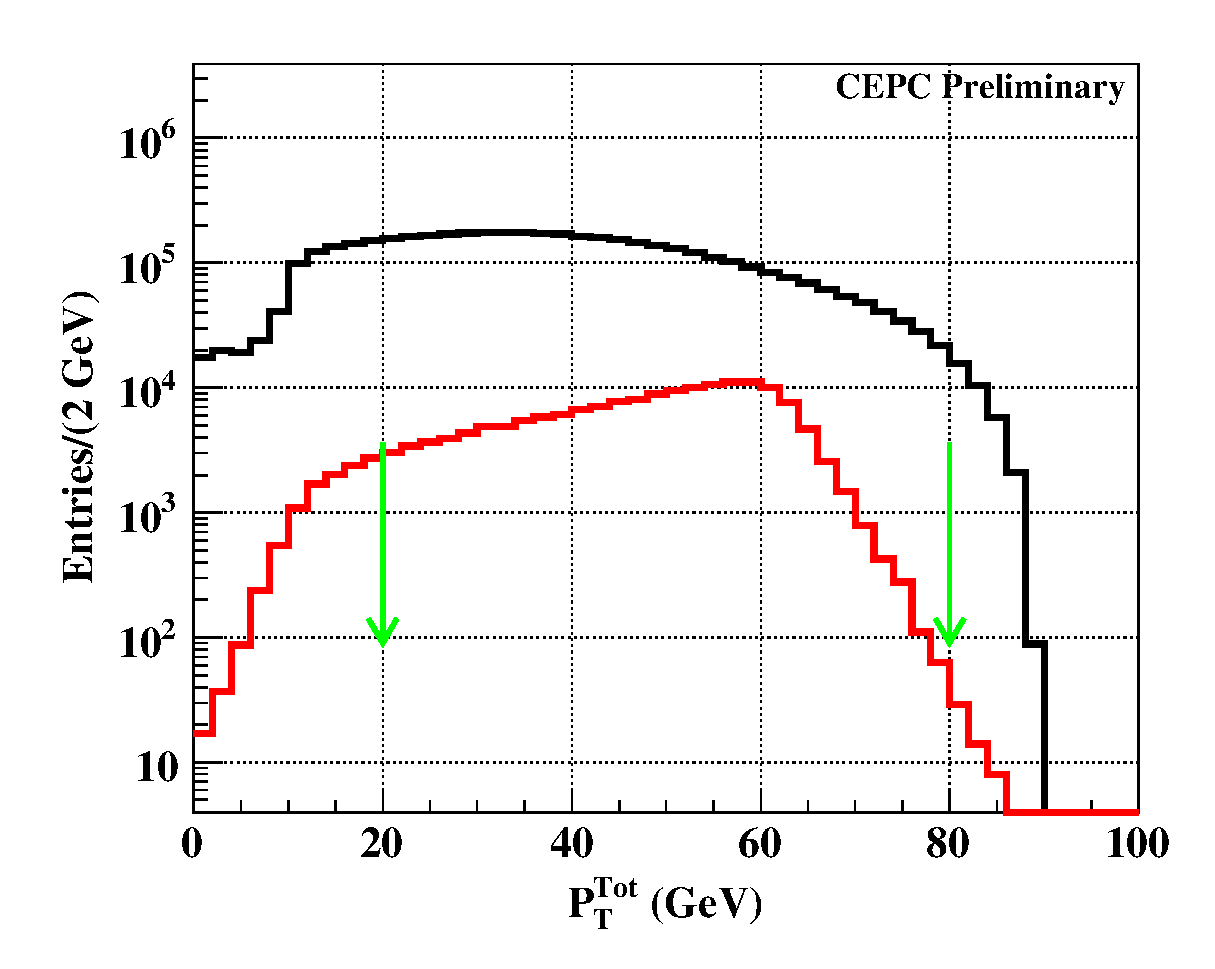
\includegraphics[width=0.35\textwidth]{filterfig/fullsim/nnH/TotalPt}
		\label{fig:uuHfilteredRecMass}
	}
	\caption[]{The distribution of missing mass, total mass and total transverse momentum in full simulation. 
	Red line is the distribution of Higgs signal. Black line is the distribution of the Standard Model background.
	Top: The left is missing mass of system. The right is total mass of system.
	Bottom: It is the distribution of total transverse momentum of system.}
	\label{fig:nnHfiltered}
\end{figure}
\begin{table}[H]
  \begin{center}
  \begin{tabular}{|c|c|c|}
  \hline \hline
  Process of signal								&				$\nu\nu H$\\
  \hline
  \multirow{3}{*}{conditions of pre-selection}	&	$65\gev/c^2 < M_{Mis} < 225\gev/c^2$	\\
  												&	$M_{Tot} > 50\gev/c^2$\\
												&	$10\gev/c < p_{T} < 100\gev/c$	\\
  \hline
  \multirow{3}{*}{conditions of validation}		&	$75\gev/c^2 < M_{Mis} < 150\gev/c^2$	\\
  												&	$100\gev/c^2 < M_{Tot} < 150\gev/c^2$	\\
												&	$20\gev/c < p_{T} < 80\gev/c$	\\
  \hline \hline
  \end{tabular}
  \caption[]{Conditions of pre-selection in MC and validation in full simulation of $\nu\nu H$ procecss}
  \label{tab:nnhprecut}
 \end{center}
\end{table}
As shown in Figure~\ref{fig:nnHfilter}, the distributions of signal and background are similar, so we should be careful to do filter 
to reject bias, and we choose the conditions as shown in Table~\ref{tab:nnhprecut}. 
Percent of each channel has changed after pre-selection, but it makes sense for analysis.

After reconstructed, we can get distribution of the same variables, as shown in Figure~\ref{fig:nnHfiltered}.
Considering the resolution of detector in full simulation, the conditions of validation should be more strict.

%\subsection{Reconstruction software !!!!!!!!!!!!!!!!!!!!!!!!!!!}
%Arbor is a reconstruction software for CEPC. 
%In Table~\ref{tab:RecEffLep}, we show the reconstruction efficiency of leptons by Arbor. The reconstruction efficiency of electron is near 
%90\%, and of the muon is near 98\%.
%\begin{table}[H]
%  \begin{center}
%  	\begin{tabular}{|c|c|c|c|c|c|}
%      \hline \hline
%	  $Z$ boson decay & $W$ boson decay & Excepted	&	Yield & Observable	&	Efficiency	\\ 
%      \hline
%	  \multirow{5}{*}{$\mu^+\mu^-$}		& $e\nu e\nu$		&  89	&   88	&  76	&	86\%\\
%	  									& $\mu\nu\mu\nu$	&  87	&   89	&  80	&	90\% \\
%	  									& $e\nu\mu\nu$		&  176	&	174 &  157	&	90\% \\
%	  									& $e\nu q\bar{q}$	&  1117	&  1105	& 1042	&	94.3\%\\
%	  									& $\mu\nu q\bar{q}$	&  1106	&  1110	& 1056	&	95.1\%\\
%	  \hline
%	  \multirow{5}{*}{$e^+e^-$}			& $e\nu e\nu$ 	 	&  95	&	91	&  62	&	68\%\\
%	  									& $\mu\nu\mu\nu$ 	&  94	&	82	&  63	&	77\% \\
%	  									& $e\nu\mu\nu$	 	&  188	&	178 &  132	&	74\% \\
%	  									& $e\nu q\bar{q}$	&  1195	&	1182& 1041	&	80.1\% \\
%	  									& $\mu\nu q\bar{q}$	& 1184	&	1221& 1194	&	80.0\% \\
%      \hline \hline
%    \end{tabular}
%   \caption[Monte Carlo purities in the single lepton sample]{Resonstruction efficiency of leptons in each decay channels. Excepted is the 
%   number of the theoretical events. Yield is the number of real generation events. Observable is the number of true events 
%   after leptons' and jets' number selection. The efficiency is observable over yield.}
%  \label{tab:RecEffLep}
% \end{center}
%\end{table}

\section{Measurement of $Br(H\rightarrow WW^*)$}
After pre-selection, the fundamental for measurement of branch ratio is complete. Just as the mentioned before, here are too many subchannels
to be described in detail, so sone typical subchannels should be represented below. 

\subsection{Analysis of $e^+e^-\rightarrow ZH, Z\rightarrow\mu^+\mu^-, H\rightarrow WW^*, WW^*\rightarrow e\nu\mu\nu$ decay}
\subsubsection{Event selection}
It is a chosen channel because only two visible particles in final states from $W$ bosons.
Therefore, the background would be supressed effectively by different lepton flavors.
And only leptonic decay of $b$-jets, $W$ boson and $\tau$ would be survived.

Refered to the Moxin's article~\ref{}, only few number of $ZZ\rightarrow \mu^+\mu^-\tau^+\tau^-$ decay and $ZZ\rightarrow 4\tau$ decay 
would not be rejected by requiring three muons and one electron and number of remain particles are less than 3. 
So the Higgs background would be main background compared to the Standard Model background.

Furthermore, the spatial resolution of vertex detector(VTX) of CEPC 
constructed with high resolution pixel sensors near the interacted point(IP) is better than 3 $\mu$m,
so leptonic decay of $\tau$  and $b\text{-}$jet would be rejected effectively by a constructed function, which is 
$\sqrt{(\frac{D_{0}}{sigD_{0}})^2+(\frac{Z_{0}}{sigZ_{0}})^2} < 5$. 
\begin{figure}[H]
\centering
	\subfigure[]{
		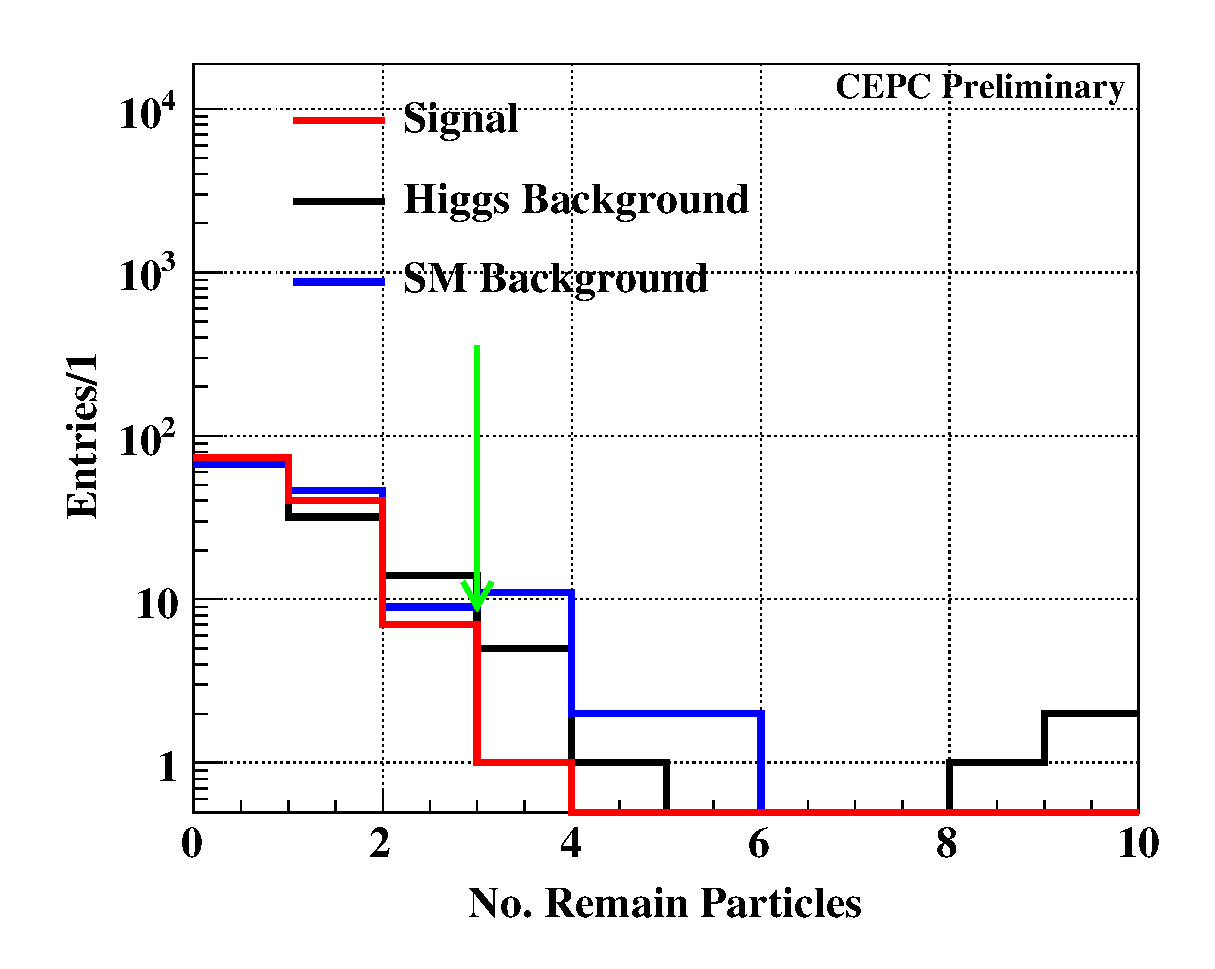
\includegraphics[width= 0.35\textwidth]{e2e2H/evuv/nRem}
		\label{fig:euRem}
	}
\subfigure[]{
	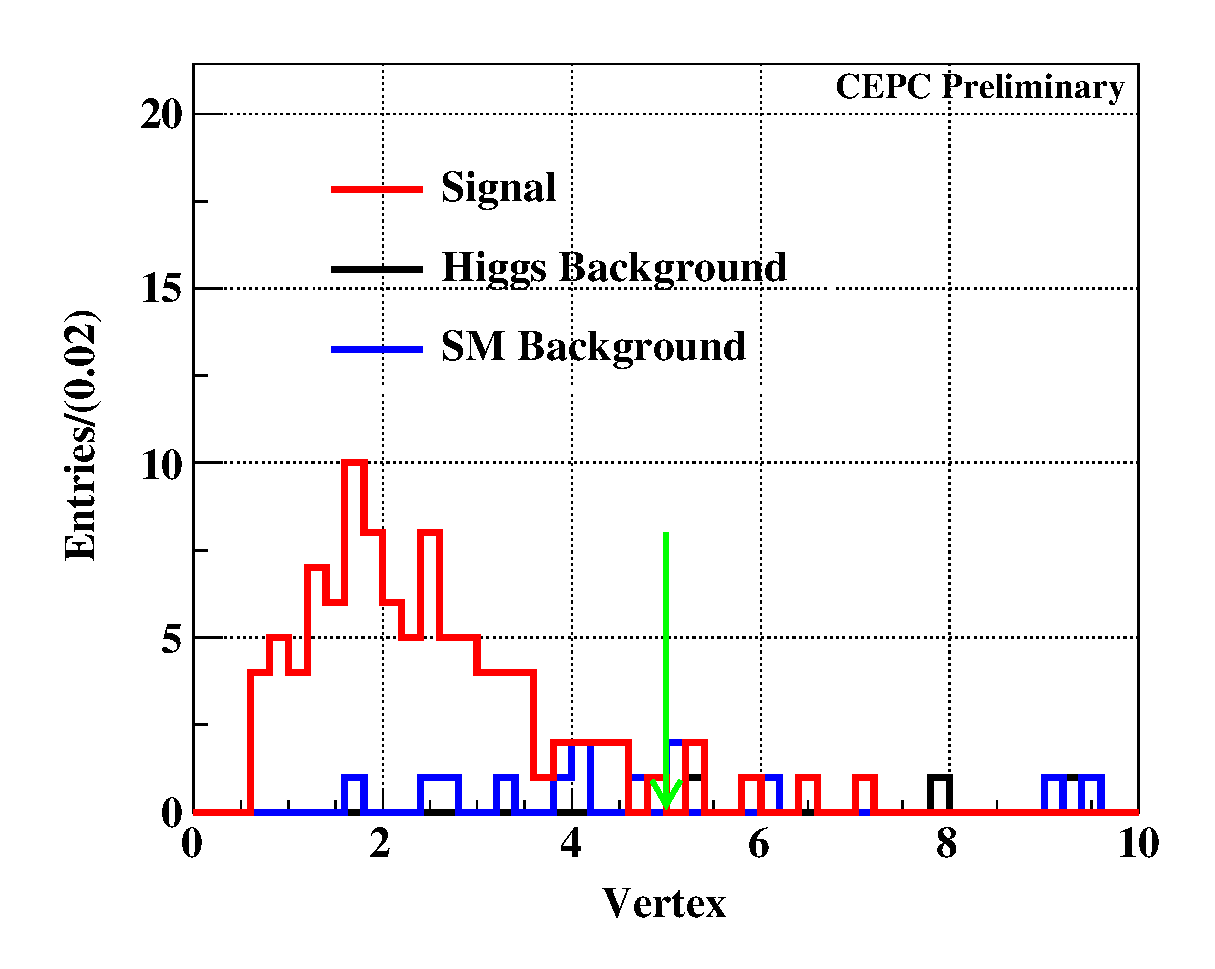
\includegraphics[width= 0.35\textwidth]{e2e2H/evuv/Vertex}
	\label{fig:euVertex}
}
\caption[]{\ref{fig:euRem} The No. remain particles of $e^+e^-\rightarrow ZH, Z\rightarrow\mu^+\mu^-, H\rightarrow WW^*,  
	WW^*\rightarrow e\nu\mu\nu$ decay. Except for four tracks, there are few photons, so we can veto semi-leptonic decay
	and hadronic decay of background.
	\ref{fig:euVertex} The distribution of Vertex of $e^+e^-\rightarrow ZH, Z\rightarrow\mu^+\mu^-, H\rightarrow WW^*, 
	WW^*\rightarrow e\nu\mu\nu$ decay. And there are two leptons totally from $W$ boson, so we plus the value of each lepton.
	And leptons from $\tau$ and $b$-jet would fly a long distance, so they would be rejected effectively.}
\label{fig:euRemandVertex}
\end{figure}

After event selection in, final number of events of signal and background are in Table~\ref{tab:emu}. And the main background of this channel is 
 $e^+e^-\rightarrow  ZZ\rightarrow\tau^+\tau^-\mu^+\mu^- $, as shown in Table~\ref{tab:uueubkg}.
\begin{table}[H]
\begin{center}
\begin{tabular}{cccc}
\hline \hline
\multicolumn{1}{c}{Category} & \multicolumn{1}{c}{Signal}&\multicolumn{1}{c}{$ZH$ background}&\multicolumn{1}{c}{SM background}\\   
\hline
  Total                                                 &     172   & 34624 &700311\\
  Validation of pre-selection				            &     136   & 29263 & 117395\\
  $N_{ZPole}=2; N_{Isolep}=2; l_1 = e, l_2 = \mu$       &     122   &   145 &   150  \\
  $N_{Remain} < 3$                                      &     121   &   113 &   122   \\
  $10\gev < M_{Inv}^{e\mu} < 65\gev$                    &     116   &   101 &   87  \\
  $M_{Missing} < 65\gev/c^2$                      		&     110   &   26  &   36   \\
  $\sqrt{(\frac{D0}{sigD0})^2+(\frac{Z0}{sigZ0})^2} < 5$&     93    &   3   &   10   \\
  \hline \hline
  \end{tabular}
  \caption[Monte Carlo purities in the single lepton sample]{% Monte
	  The final event selection of $e^+e^-\rightarrow ZH, Z\rightarrow\mu^+\mu^-, H\rightarrow WW^*, WW^*\rightarrow e\nu\mu\nu$ decay.}
\label{tab:emu}
\end{center}
\end{table}
\begin{table}[H]
\begin{center}
\begin{tabular}{lrc}
\hline\hline
Decay Chain	& Final States 	&	Number of Events\\
\hline
$e^+e^-\rightarrow ZZ, ZZ\rightarrow\tau^+\tau^-\mu^+\mu^- $	& $\mu^+, \mu^-, \tau^+, \tau^-$			&10	\\
\hline\hline
\end{tabular}
\caption{Summery of total background with the same final states of signal event}
\label{tab:uueubkg}
\end{center}
\end{table}

\subsubsection{Statistical result}
After selection, we can get the distribution of recoil mass of $\mu^+\mu^-$, as shown in Figure~\ref{fig:uuhevuvrecfit}.
\begin{figure}[H]
\centering
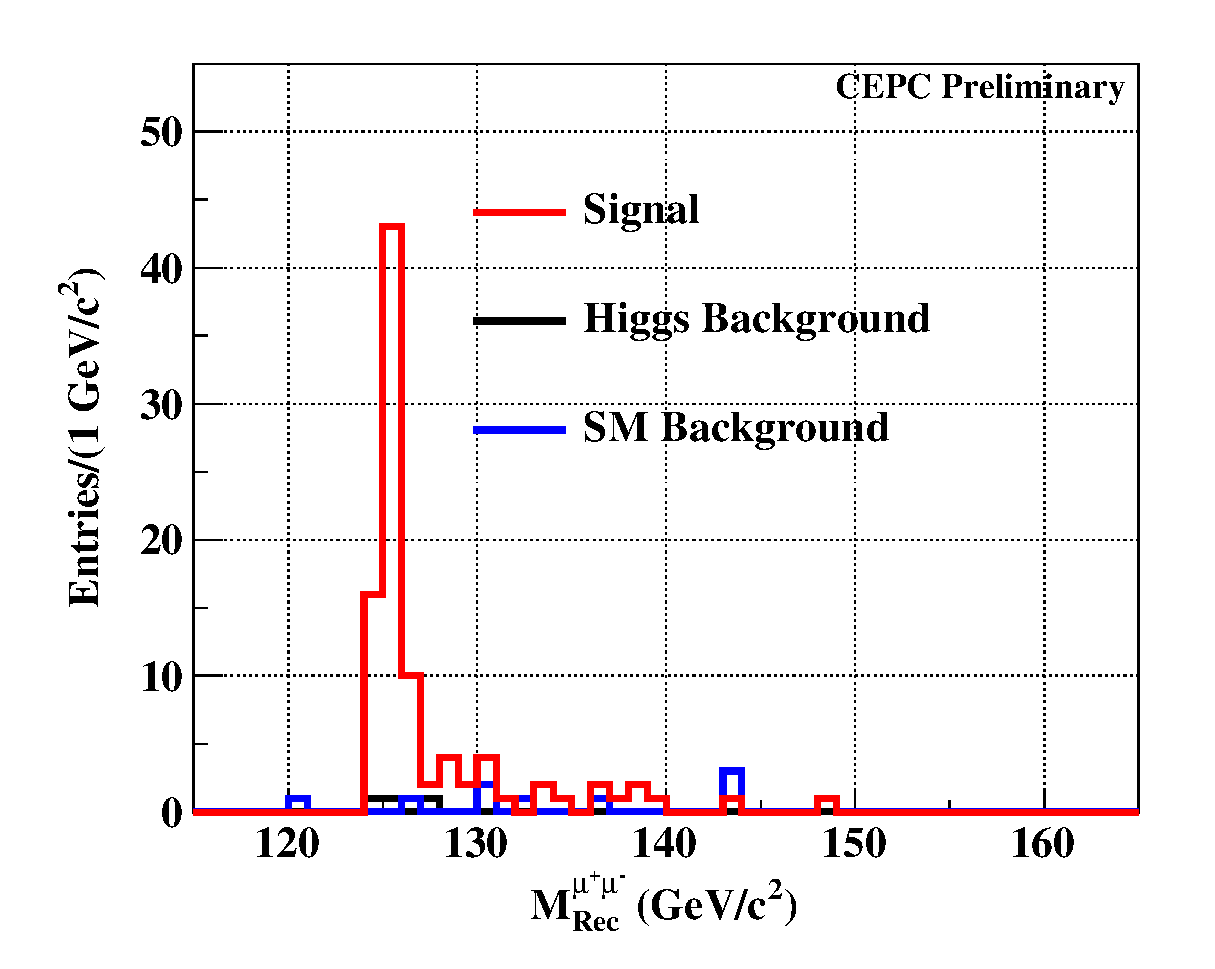
\includegraphics[width=0.5\textwidth]{e2e2H/evuv/uuh_recfit}
\label{fig:uuhevuvrecfit}
\caption[]{The distribution of recoil mass of $\mu^+\mu^-$ after event selection}
\end{figure}

Number of signal events could be got by counting,
\begin{equation*}
N_{sig} = 93\pm10 ;
\end{equation*}
and $N_{sig}$ is events of signal, the effeciency of selection $\varepsilon = 54.1\%$. Statistical uncertainty is 
\begin{equation*}
Accu.=\frac{\sqrt{S+B}}{S} = 11\%.
\end{equation*}

\subsection{Analysis of $e^+e^-\rightarrow ZH, Z\rightarrow e^+e^-, H\rightarrow WW^*, WW^*\rightarrow \mu\nu q\bar{q}$ decay}
\subsubsection{Event selection}
In this subchannel, number of signal events is much more lager than full-leptonic decay subchannel 
although it's not as clear as $e\nu\mu\nu$ channel,
so we could get a higher accuracy. 
The final states in this subchannel are three leptons, several jets and neutrinoes which are perfomanced as missing mass.
Full-leptonic decay background of $\tau$ events would be rejected by number of remain particle less than 30 and larger than 7. 

As mentioned before, invariant mass and corresponding recoil mass of two leptons from initial $Z$ boson are effective criteria 
to supress the Standard Model background.
So validation of pre-selection, $80\gev/c^2 < M_{Inv}^{e^+e^-} < 100\gev/c^2$ and $120\gev/c^2 < M_{Rec}^{e^+e^-} < 150\gev/c^2$ are applied.

The jets come from diffenert ways,such as Higgs decay, $W$ boson decay, $Z$ boson decay and $\tau$ decay.
Based on this, the invariant mass of jets, $10\gev/c^2 < M_{Rec}^{di-Jet} < 95\gev/c^2 $, could distinguish the signal and background well. 
And $b$-jet would not come from $W$ boson, so we could use $b$-tagging to vote the $b$-jet background.

In signal, here is only one isolated muon from $W$ boson and its start point is near the IP, so background 
of muon from $\tau$ or jet could be rejected powerfully by a function. The form of this function is similar with before, 
$\sqrt{(\frac{D_{0}}{sigD_{0}})^2+(\frac{Z_{0}}{sigZ_{0}})^2} < 4$.
In order to veto background of t channel, transverse momentum $p_T > 5\gev$ has applied.
\begin{figure}[H]
\centering
	\subfigure[]{
		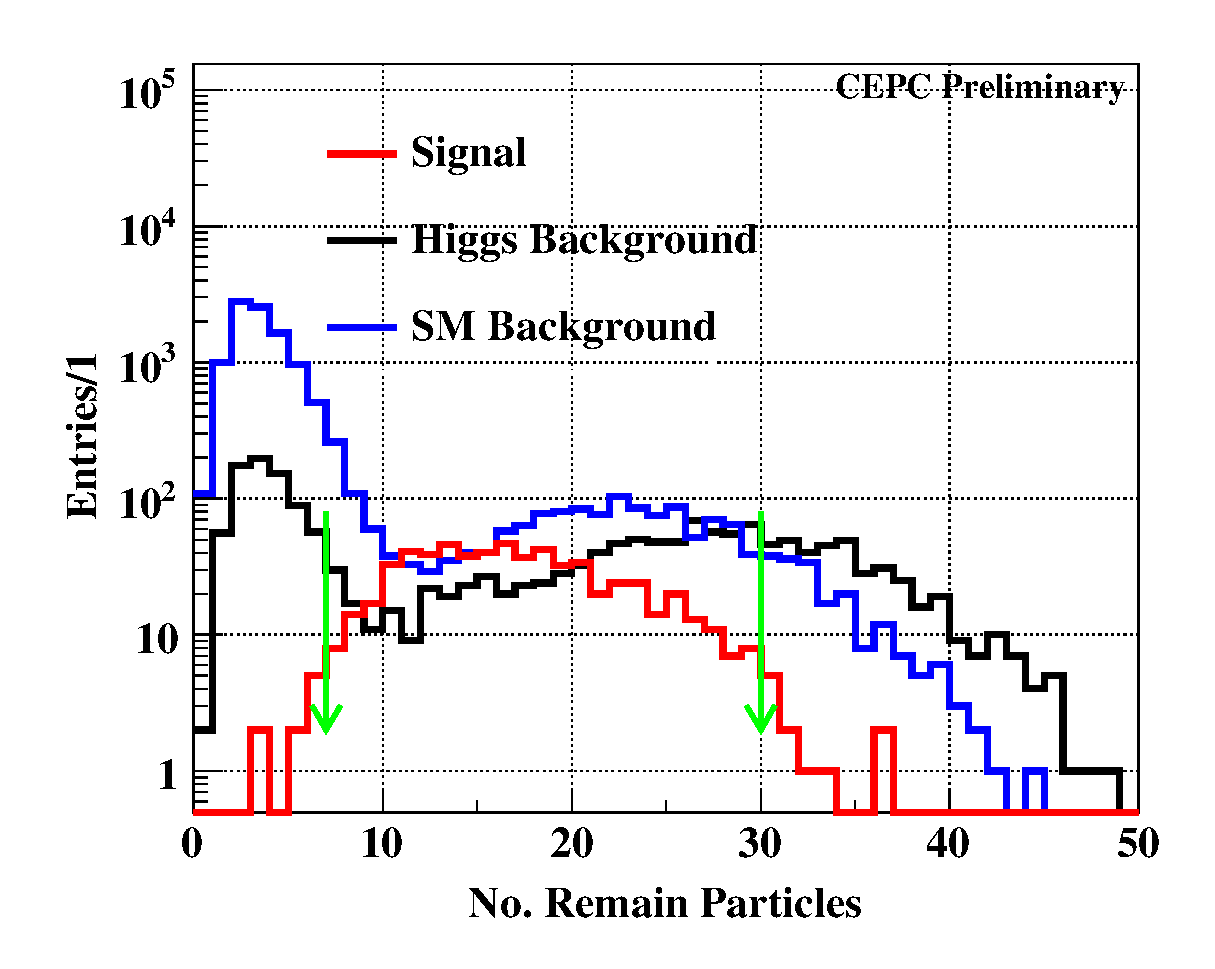
\includegraphics[width= 0.35\textwidth]{e1e1H/uvqq/nRem}
		\label{fig:eeuvqqRem}
	}
\subfigure[]{
	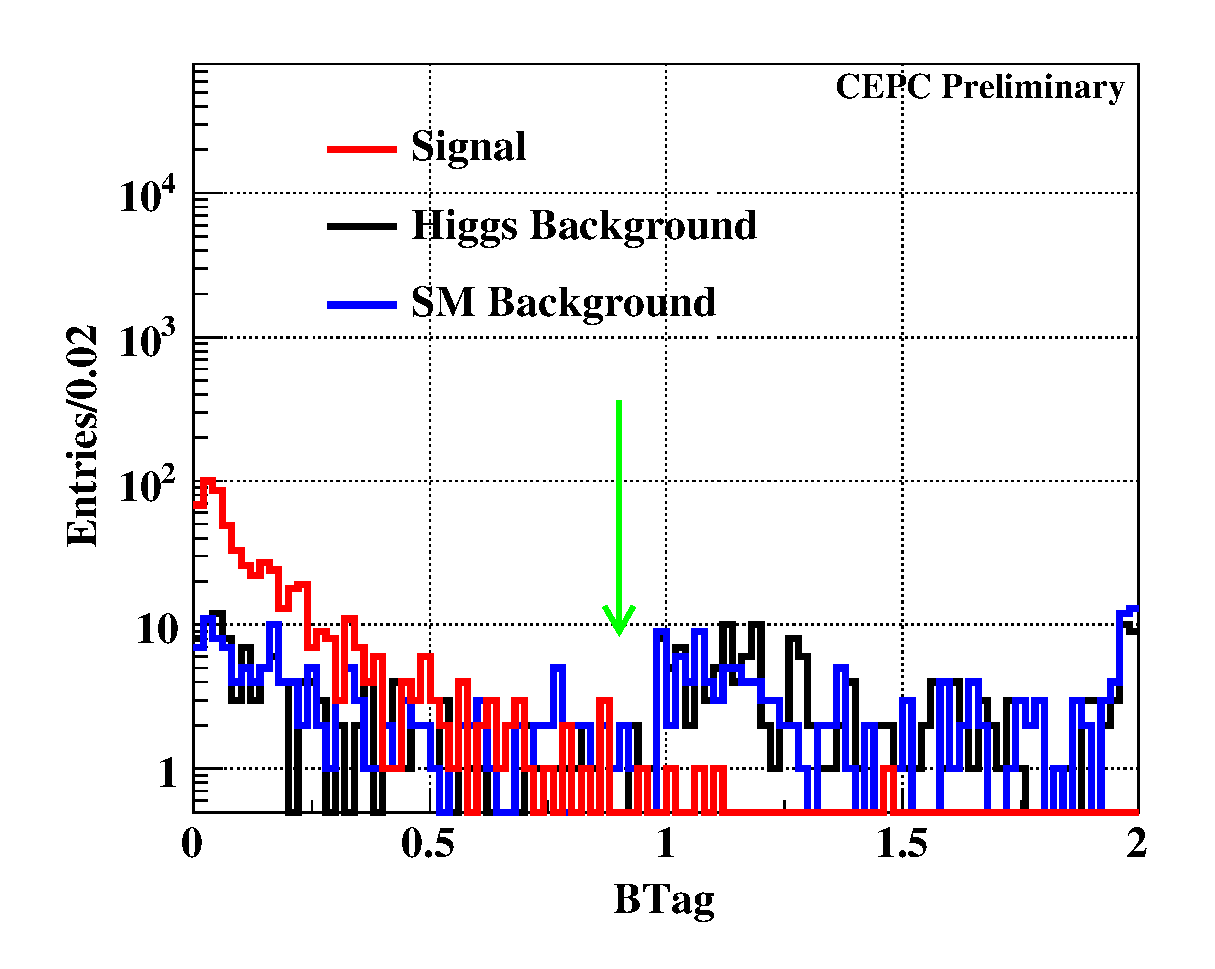
\includegraphics[width= 0.35\textwidth]{e1e1H/uvqq/Btag}
	\label{fig:eeuvqqBtag}
}
\subfigure[]{
	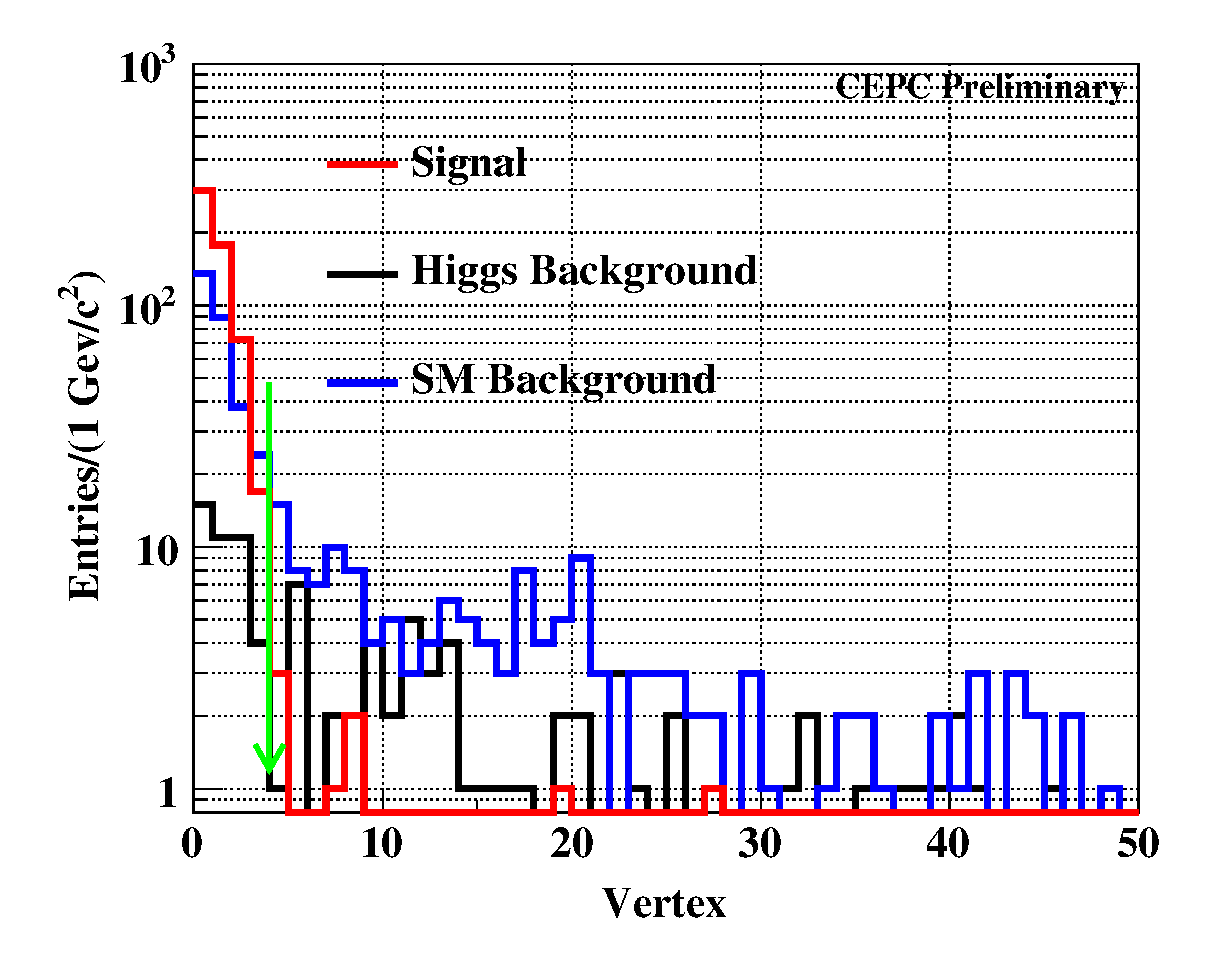
\includegraphics[width= 0.35\textwidth]{e1e1H/uvqq/Vertex}
	\label{fig:eeuvqqVertex}
}
\subfigure[]{
	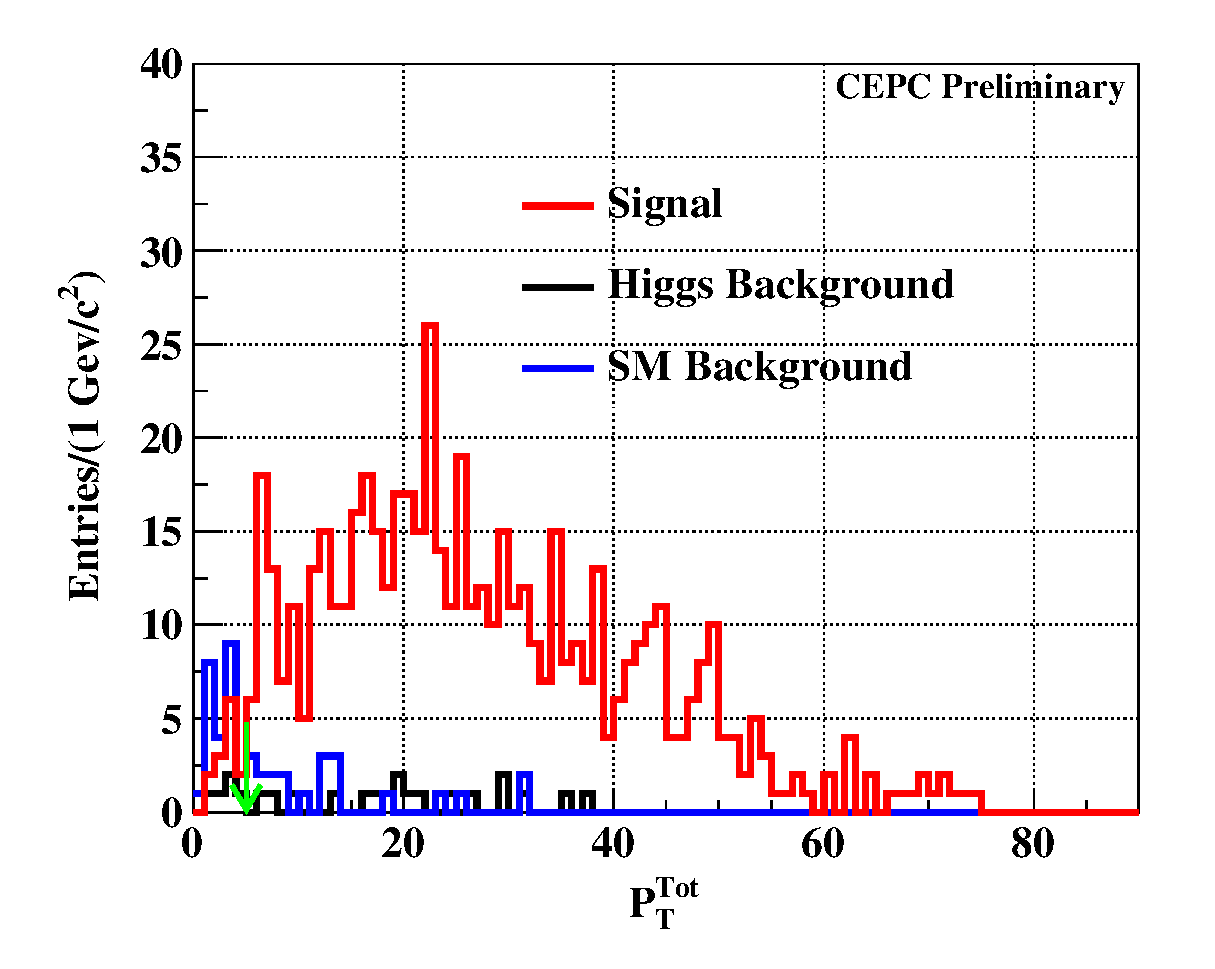
\includegraphics[width=0.35\textwidth]{e1e1H/uvqq/Pt}
	\label{fig:eeuvqqPt}
}
\subfigure[]{
	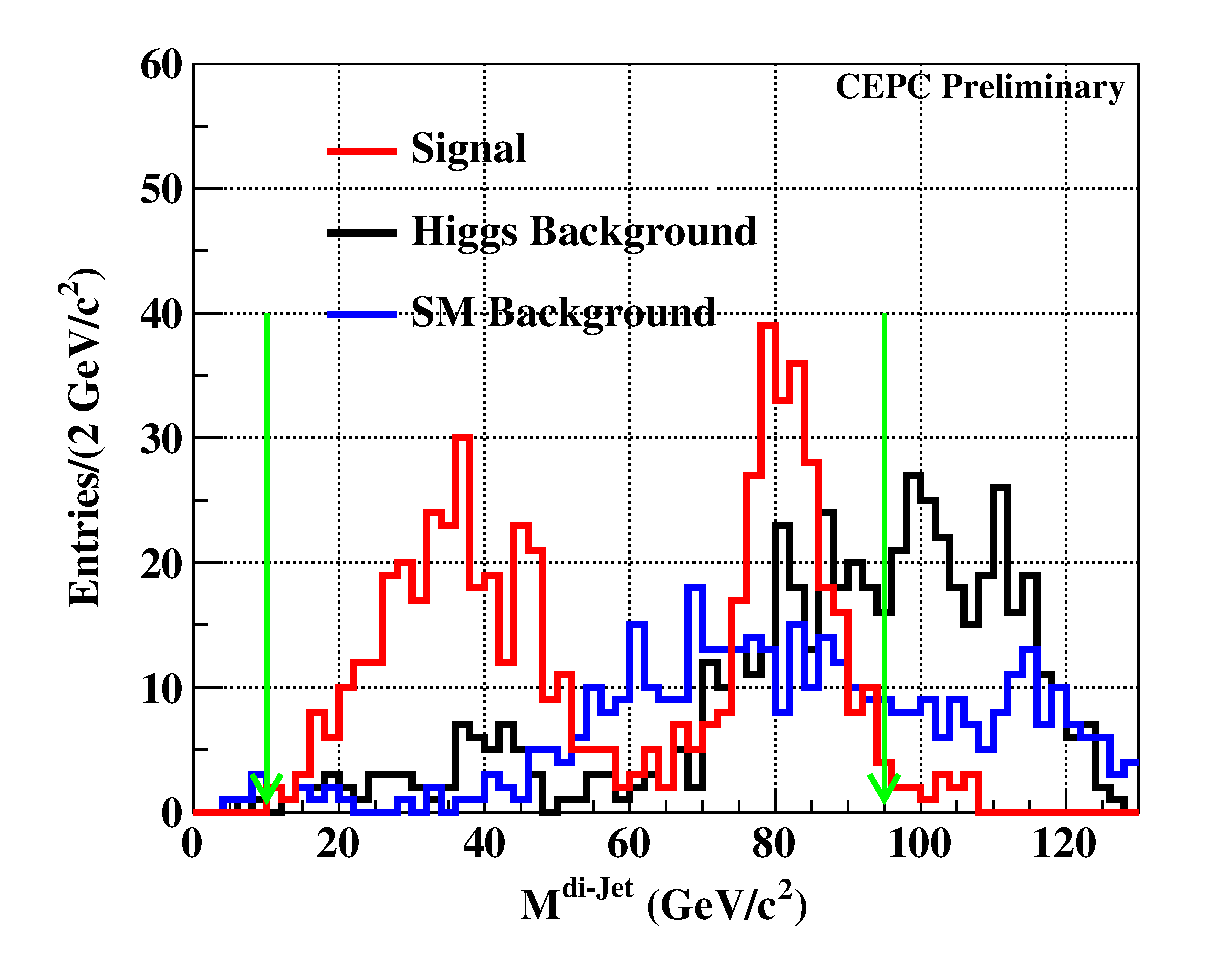
\includegraphics[width= 0.35\textwidth]{e1e1H/uvqq/diJet_InvMass}
	\label{fig:eeuvqqInvJet}
}
\caption[]{
	\ref{fig:eeuvqqRem} The No. remain particles of $e^+e^-\rightarrow ZH, Z\rightarrow e^+e^-, H\rightarrow WW^*,  
	WW^*\rightarrow \mu\nu q\bar{q}$ decay. 
	Because it is semi-leptonic decay channel, so the No. remain particles should between it of hadronic decay and full-leptonic decay.
	\ref{fig:eeuvqqBtag} The distribution of Btag, we plus the Btag value of each jets because of existing two jets. And because no $b$-jet 
	decay from $W$ boson, the value of them should be less than 1.
	\ref{fig:eeuvqqVertex} The distribution of vertex of lepton. Leptons from $\tau$ and $b$-jet would fly a long distance, 
	so they would be rejected effectively.
	\ref{fig:eeuvqqPt} The distribution of transverse momentum $p_T$. Transverse momentum of t channel would be lower than of s channl.
	\ref{fig:eeuvqqInvJet} The distribution of di-jet invariant mass, the high-side could distinguish the jets from $Z$ boson or $H$ boson.
	}
\label{fig:eeuvqqfourcut}
\end{figure}

After the selection as shown in Table~\ref{tab:eeuvqqCutchain}, the background are supressed almostly. 
Table~\ref{tab:uuuvqqbkg} shows the main background after event selection.
\begin{table}[H]
  \begin{center}
    \begin{tabular}{ccccc}
      \hline \hline
      \multicolumn{1}{c}{Category} & \multicolumn{1}{c}{Signal}&\multicolumn{1}{c}{$ZH$} background&\multicolumn{1}{c}{SM background}\\ 
      \hline
      Total 	      	 									&   1149	& 36319	& 1303847\\
      $N_{ZPole}=2; N_{Isolep}=1; N_{Jets} =2; l = \mu$		&   1022	& 1970	& 21857\\
	  Validation of pre-selection					   		&   631 	& 1207	& 2987\\
	  $7 < N_{Remain} < 30$									&	603		& 540	& 436\\
	  $15\gev/c^2 < M_{Rec}^{di-Jet} < 95\gev/c^2 $			&	589		& 284	& 278\\
	  $Btag < 0.9$											&	584		& 116	& 131\\
	  $M_{Missing} < 45\gev/c^2$							&   571		& 72	& 102\\
	  $\sqrt{(\frac{D0}{sigD0})^2+(\frac{Z0}{sigZ0})^2} < 4$&	564  	& 23 	& 45\\
	  $p_T > 5\gev$											&	551		& 18	& 21	\\	
      \hline \hline
    \end{tabular}
  \caption[Monte Carlo purities in the single lepton sample]{% Monte
    The final event selection of $e^+e^-\rightarrow ZH, Z\rightarrow e^+e^-, H\rightarrow WW^*, WW^*\rightarrow \mu\nu q\bar{q}$ decay}
  \label{tab:eeuvqqCutchain}
  \end{center}
\end{table}
\begin{table}[H]
\begin{center}
\begin{tabular}{lrc}
\hline\hline
Decay Chain	& Final States 	&	Number of Events	\\
\hline
$e^+e^-\rightarrow ZH, Z\rightarrow e^+e^-, H\rightarrow WW^*\rightarrow \tau\nu q\bar{q}$ & $e^+, e^-, \tau, \nu, 2q $	&	14\\
$e^+e^-\rightarrow e^+e^-Z, Z\rightarrow qq$ 					& $e^+, e^-, 2q$								&	13\\
\hline\hline
\end{tabular}
\caption{Summery of total background with the same final states of signal event}
\label{tab:uuuvqqbkg}
\end{center}
\end{table}

\subsubsection{Statistical result}
After selection, the distribution of recoil mass of $e^+e^-$ is shown in Figure~\ref{fig:eehuvqqrecfit}.
\begin{figure}[H]
\centering
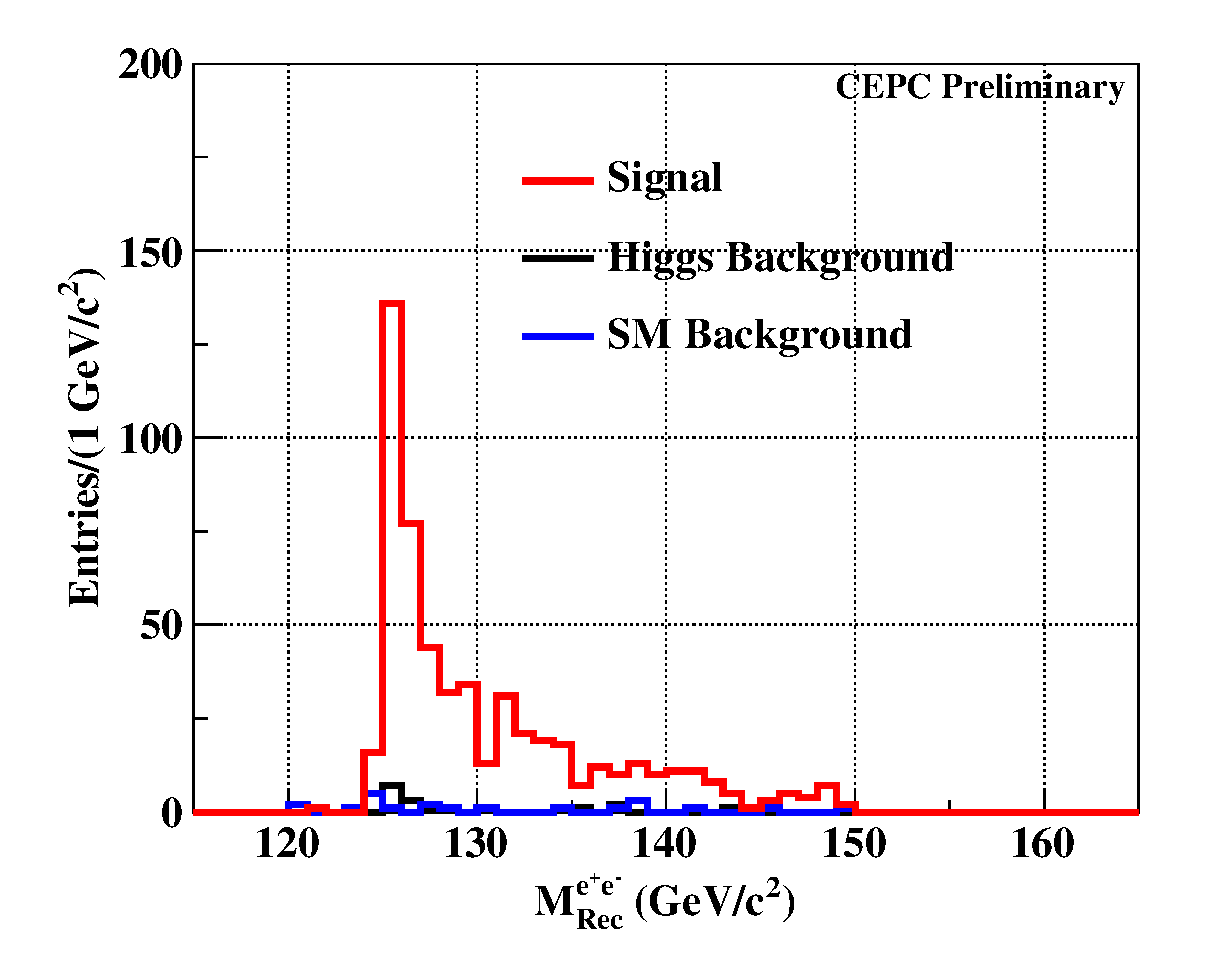
\includegraphics[width=0.5\textwidth]{e1e1H/uvqq/fit_RecMass}
\label{fig:eehuvqqrecfit}
\caption[]{The distribution of recoil mass of $\mu^+\mu^-$ after event selection}
\end{figure}

We can get the number of signal events by counting,
\begin{equation*}
N_{sig} = 551\pm24 ;
\end{equation*}
and $N_{sig}$ is events of signal, the effeciency of selection $\varepsilon = 48.0\%$. Statistical uncertainty is 
\begin{equation*}
Accu.=\frac{\sqrt{S+B}}{S} = 4.5\%.
\end{equation*}

\subsection{Analysis of $e^+e^-\rightarrow ZH, Z\rightarrow \nu\bar{\nu}, H\rightarrow WW^*, WW^*\rightarrow q\bar{q}q\bar{q}$ decay}
\subsubsection{Event selection}
This is a hadronic decay channel and no isolated lepton. Lost of the Standard Model background would not be 
supressed by no isolated lepton and at least two jets.
The number of final particles is required to be larger, $No._{Particles}^{Total} > 20$, because the final particles are 
producted a lot after hadronization of quarks. And fraction of hadronic process would be enhanced a lot by this requirement.
\begin{figure}[H]
	\centering
	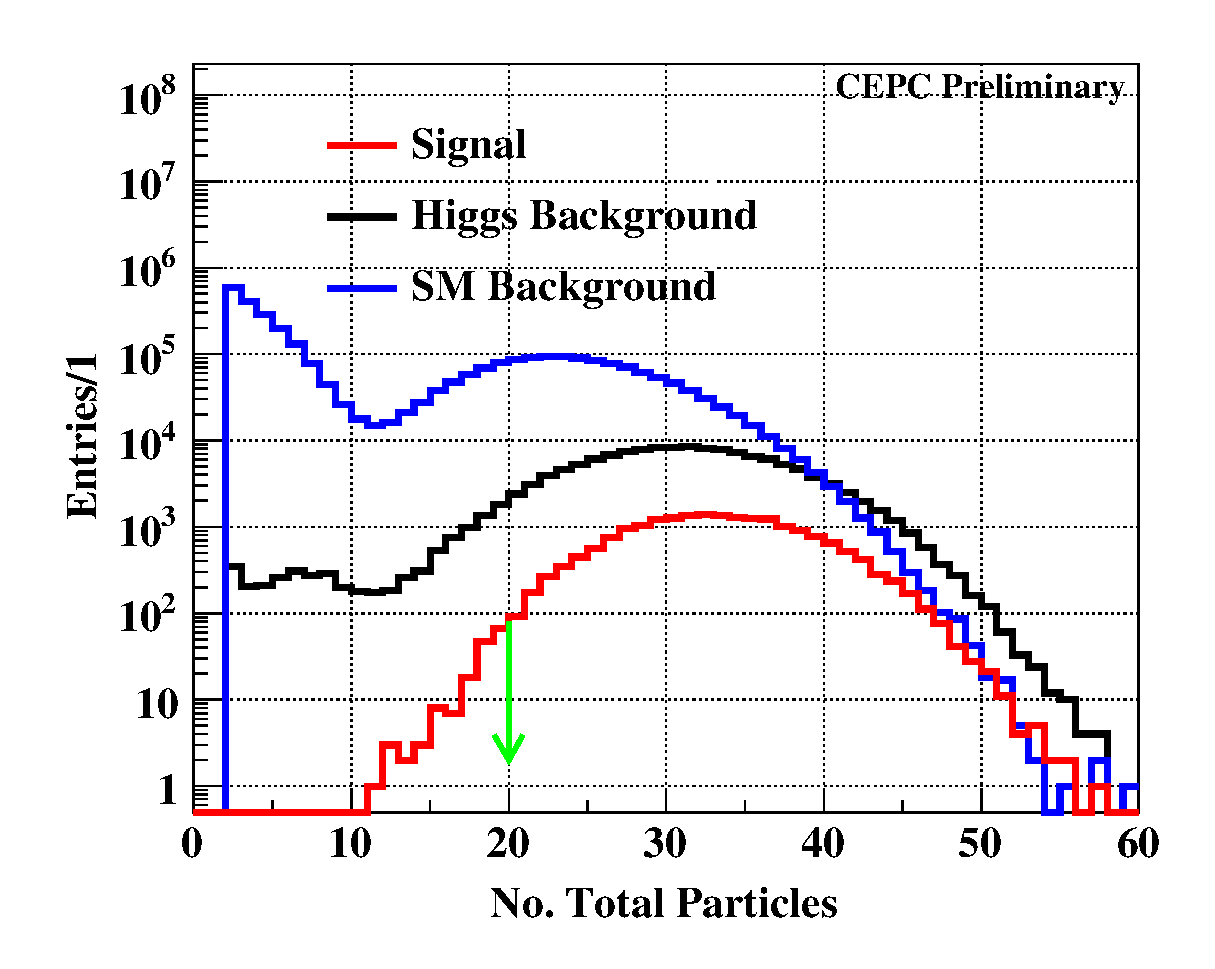
\includegraphics[width= 0.35\textwidth]{nnH/fourq/TotPart}
	\label{fig:nnH4qTotPart}
	\caption[]{The number of total final particles distribution. To count the total number, the enengy threshold of each particle 
	is required, $E > 1\gev$}
\end{figure}

The the jet clustering has been done twice. At the first time, 
two jets are clustered to reject the two jets background, such as $H\rightarrow q\bar{q}$ decay of Higgs background, 
$ZZ$ semi-leptonic decay and "single $Z-nu$" semi-leptonic decay process of the Standard Model background. 
These two jets are required $Btagging < 0.9$, $Cos\theta_{2jets} > 0.87$ and $\Sigma|M_{Inv}^{2jet}| > 50\gev/c^2$. 
And at the second time, four jets are required. In this situation, the characterizes of signal are more important. 
Y value is effective to distinguish the signal and background. The event is required to have $Y_{34} > 0.005$. 
According to these four jets, we would get two components which are the combination of four momentum of among two jets. 
The invariant mass of one of the components should be near the mass peak of the $W$ boson, and the jets in the other part 
are regard as from virtual $W$ boson decay. Figure~\ref{fig:nnHfourqFMass} shows the distribution of these two component. 
The combined functions are:
\begin{itemize}
	\item $ 65\gev/c^2 < M_{Inv}^{Real4jet} < 85\gev/c^2$;
	\item $ 15\gev/c^2 < M_{Inv}^{Virt4jet} < 50\gev/c^2$;
	\item $ M_{Inv}^{Virt4jet} > -7/3\dot M_{Inv}^{Real4jet} + \frac{605}{3}\gev/c^2$;
\end{itemize}
$M_{Inv}^{Real4jet}$ means invariant mass of two jets which are regard as jets decay from real $W$ boson. 
And $M_{Inv}^{Virt4jet}$ means invariant mass of two jets which are regard as jets decay from virtual $W$ boson.
\begin{figure}[H]
	\centering
	\subfigure[]{
		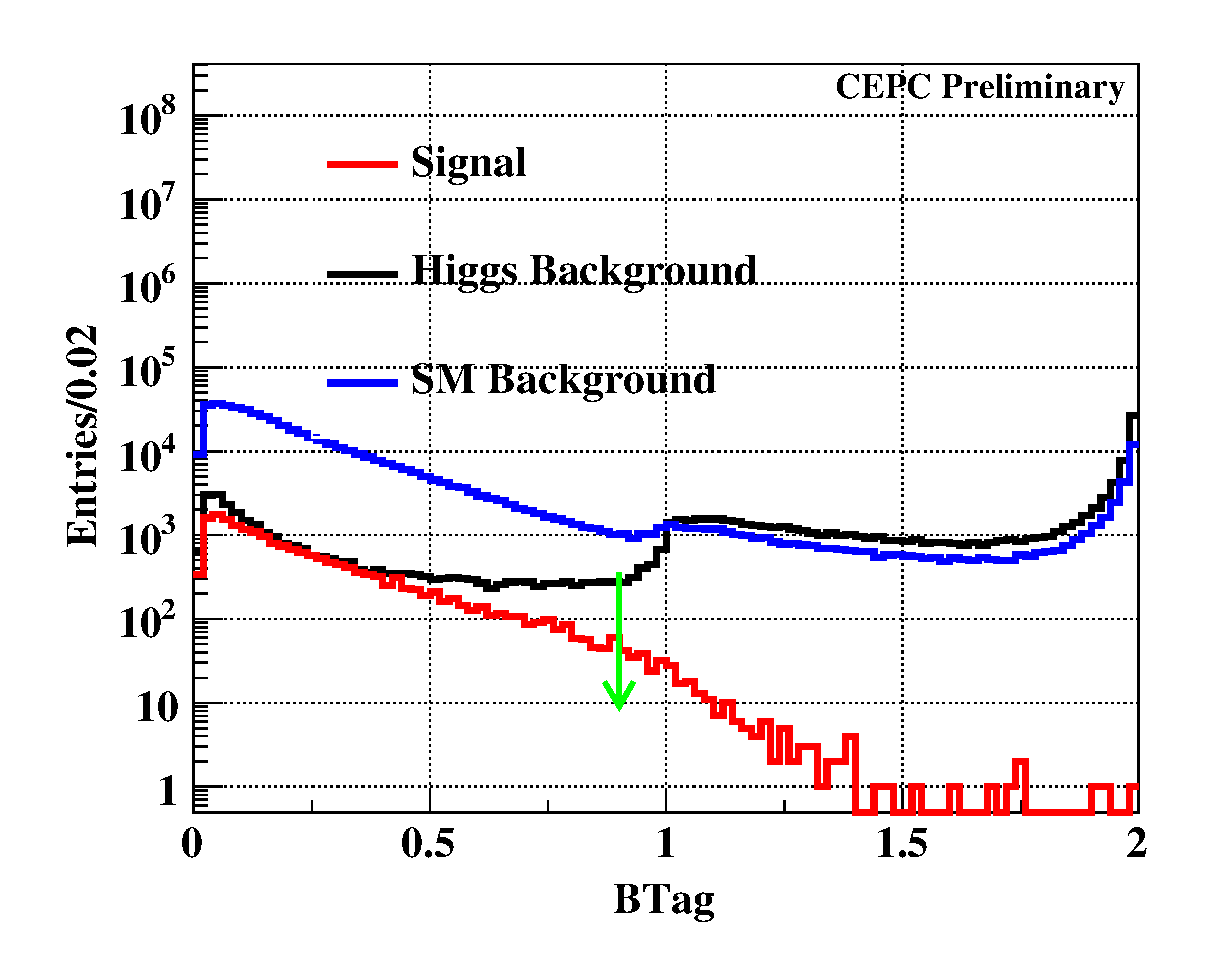
\includegraphics[width= 0.35\textwidth]{nnH/fourq/Btag}
		\label{fig:nnHfourqBtag}
	}
	\subfigure[]{
		\includegraphics[width= 0.35\textwidth]{nnH/fourq/TwoJetsAngle}
		\label{fig:nnHfourqTJAngle}
	}
	\subfigure[]{
		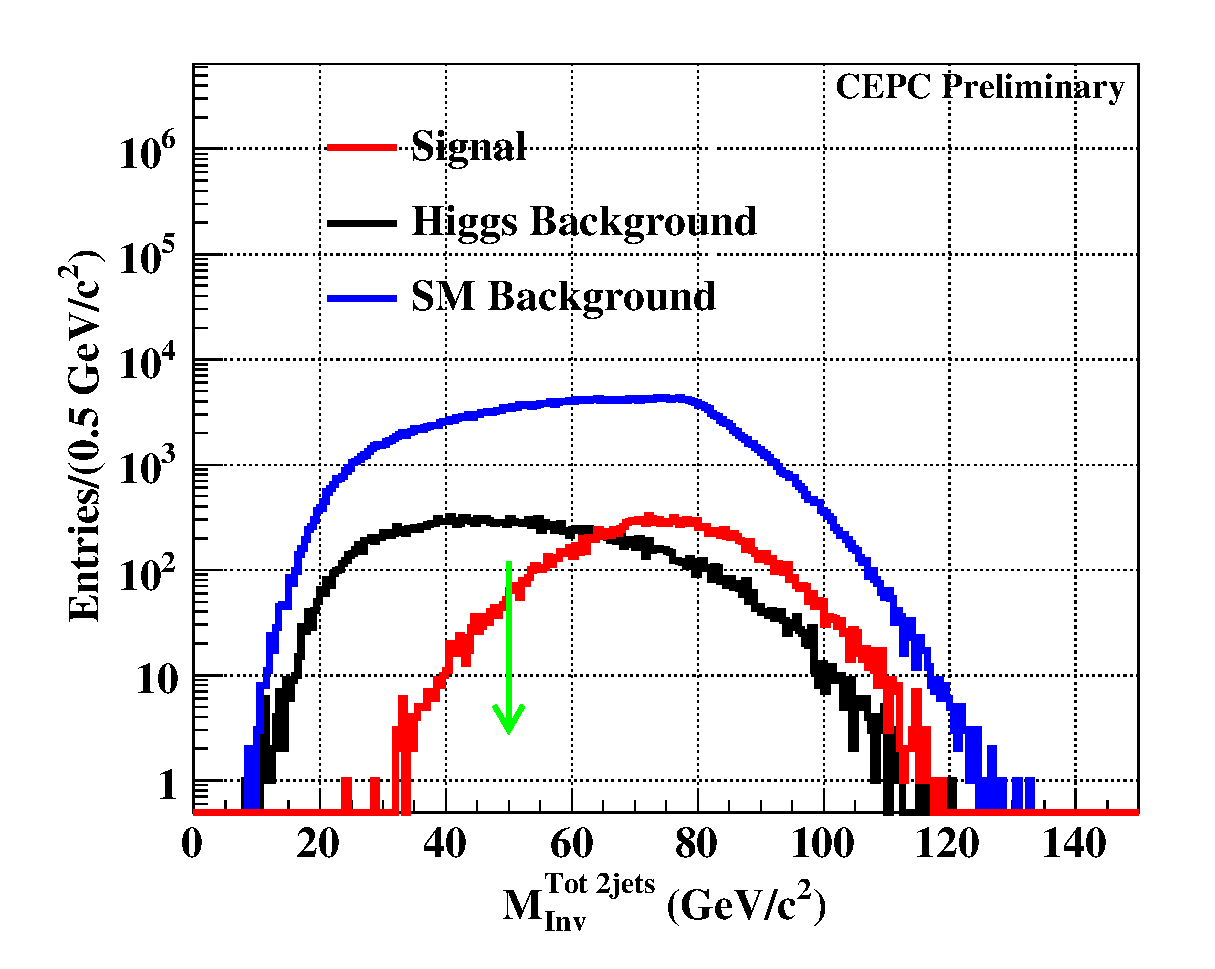
\includegraphics[width= 0.35\textwidth]{nnH/fourq/tjet_TotMass}
		\label{fig:nnHTJPInvMass}
	}
	\caption[]{
		\ref{fig:nnHfourqBtag} B-tag of two jets distribution. We plus the value of B-tag of each jet, 
		\ref{fig:nnHfourqTJAngle} The distribution of angle between two jets. The boost of Higgs is larger, so the angle 
		between two jets in signal should be smaller its in background. 
		\ref{fig:nnHTJPInvMass} The distribution of total invariant mass of two jets. The number of jets in almost background is two. 
		The invariant mass of each jet should be smaller.}
	\label{fig:nnHfourqTwoJet}
\end{figure}
\begin{figure}[H]
	\centering
	\subfigure[]{
		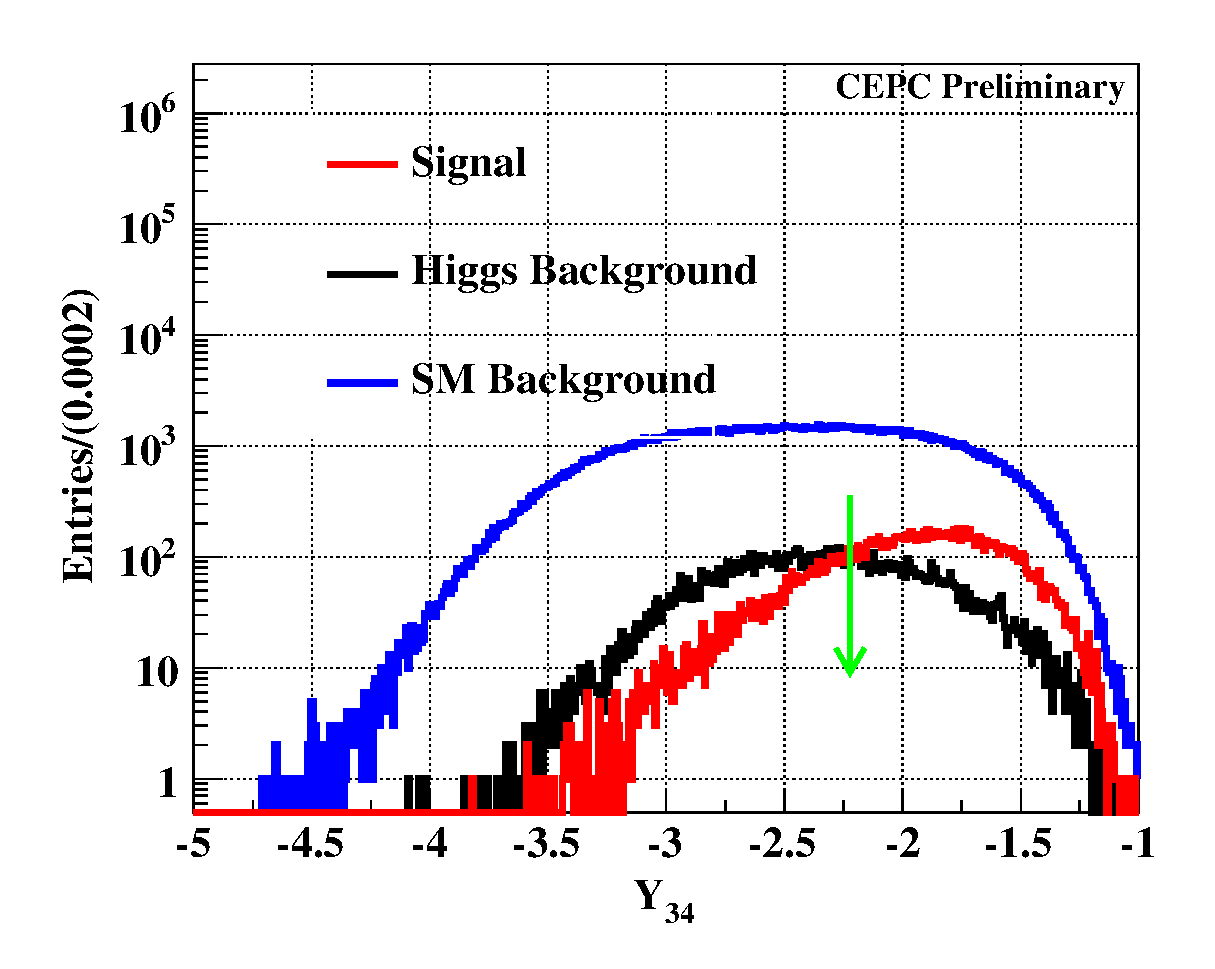
\includegraphics[width=0.35\textwidth]{nnH/fourq/Y34}
		\label{fig:nnHfourqY34}
	}
	\subfigure[]{
		\includegraphics[width=0.7\textwidth]{nnH/fourq/4qInvMass}
		\label{fig:nnHfourqFMass}
	}
	\caption[]{
		\ref{fig:nnHfourqY34} Y value distribution. 
		\ref{fig:nnHfourqFMass} 2D scatter diagram of invariant mass of real and virtual $W$ boson. The left plot representes the distribution 
		of signal, and the right is of background. In order to distinguish the signal and background effectively, a hexagonal mass window is 
		applied.}
	\label{fig:nnHfourqFourJet}
\end{figure}
%%%%%%%%%%%%%%%%%%%%%%%%%%%%%%%%%%%%%%% nn qqqq %%%%%%%%%%%%%%%%%%%%%%%%%%%%%%%%%%%%%%%%%%%%%%%

After the event selection, the signal is protected near 50\% as shown in Table~\ref{tab:nnHfourqcutchain}
\begin{table}[H]
  \begin{center}
    \begin{tabular}{cccccccc}
      \hline \hline
      \multicolumn{1}{c}{Category}      & \multicolumn{1}{c}{Signal}&\multicolumn{1}{c}{$ZH$ background}&\multicolumn{1}{c}{SM background}\\ 
      \hline
      Total 	      	 					&   23938& 208200&	21314314	\\
	  Validation of pre-selection		  	&   20405& 143765&	3166923	\\
	  $N_{Particle}^{Tot} > 20$				&	19681& 124112& 	537839	\\
	  $Btag < 0.9$							&	19349& 28857 & 	477099	\\
	  $Cos\theta_{2jets} > 0.87  $			&	19298& 28673 &	433563	\\
	  $\Sigma|M_{Inv}^{2jet}| > 50\gev$		&   18621& 14793 &	309919	\\
	  $Y_{34} > 0.005$						&	15183& 6919  &  122866	\\
	  Combined Variable						&	9022 & 3075  &	38226	\\
      \hline \hline
    \end{tabular}
  \caption[Monte Carlo purities in the single lepton sample]{% Monte
  The final event selection of $e^+e^-\rightarrow ZH, Z\rightarrow \nu\bar{\nu}, H\rightarrow WW^*, WW^*\rightarrow q\bar{q}q\bar{q}$ decay}
  \label{tab:nnHfourqcutchain}
  \end{center}
\end{table}
\begin{table}[H]
\begin{center}
\begin{tabular}{lrc}
\hline\hline
Decay Chain	& Final States 	&	Number of Events\\
\hline
$e^+e^-\rightarrow ZH, Z\rightarrow \nu\bar{\nu}, H\rightarrow c\bar{c}$ & $\nu, \bar{\nu}, c, \bar{c}$			&192	\\
$e^+e^-\rightarrow ZH, Z\rightarrow \nu\bar{\nu}, H\rightarrow b\bar{b}$ & $\nu, \bar{\nu}, b, \bar{b}$			&352	\\
$e^+e^-\rightarrow ZH, Z\rightarrow \nu\bar{\nu}, H\rightarrow gg$ 		 & $\nu, \bar{\nu}, 2g		  $			&2028	\\
$e^+e^-\rightarrow ZH, Z\rightarrow \nu\bar{\nu}, H\rightarrow ZZ^*, ZZ^*\rightarrow q\bar{q}q\bar{q}$ &
																$\nu, \bar{\nu}, 2q, 2\bar{q}$&		439\\	
$e^+e^-\rightarrow ZZ, ZZ\rightarrow \nu\bar{\nu}q\bar{q}$      & $\nu, \bar{\nu}, q, \bar{q}$					&3115	\\
$e^+e^-\rightarrow ZZ, ZZ\rightarrow \tau^+\tau^-q\bar{q}$ 		& $\tau^+, \tau^-, q, \bar{q}$					&910	\\
$e^+e^-\rightarrow WW, WW\rightarrow \tau\nu q\bar{q}$        	& $\tau, \nu, q, \bar{q}$						&	30398\\
$e^+e^-\rightarrow WW, WW\rightarrow \mu\nu q\bar{q}$        	& $\mu, \nu, q, \bar{q}$						&	277\\
$e^+e^-\rightarrow \nu\bar{\nu} Z, Z\rightarrow q\bar{q}$ 		& $\nu, \bar{\nu}, q, \bar{q}$					&	1838\\
$e^+e^-\rightarrow e\nu W, W\rightarrow e\nu q\bar{q}$        	& $e, \nu, q, \bar{q}$							&	1398\\
$e^+e^-\rightarrow qq$											& $2q$											&262 \\
\hline\hline
\end{tabular}
\caption{Summery of main background with the same final states of signal event}
\label{tab:nnqqqqbkg}
\end{center}
\end{table}

\subsubsection{Statistical result}
After selection, we can get the distribution of missing mass, as shown in Figure~\ref{fig:nnhqqqqmismass}.
\begin{figure}[H]
\centering
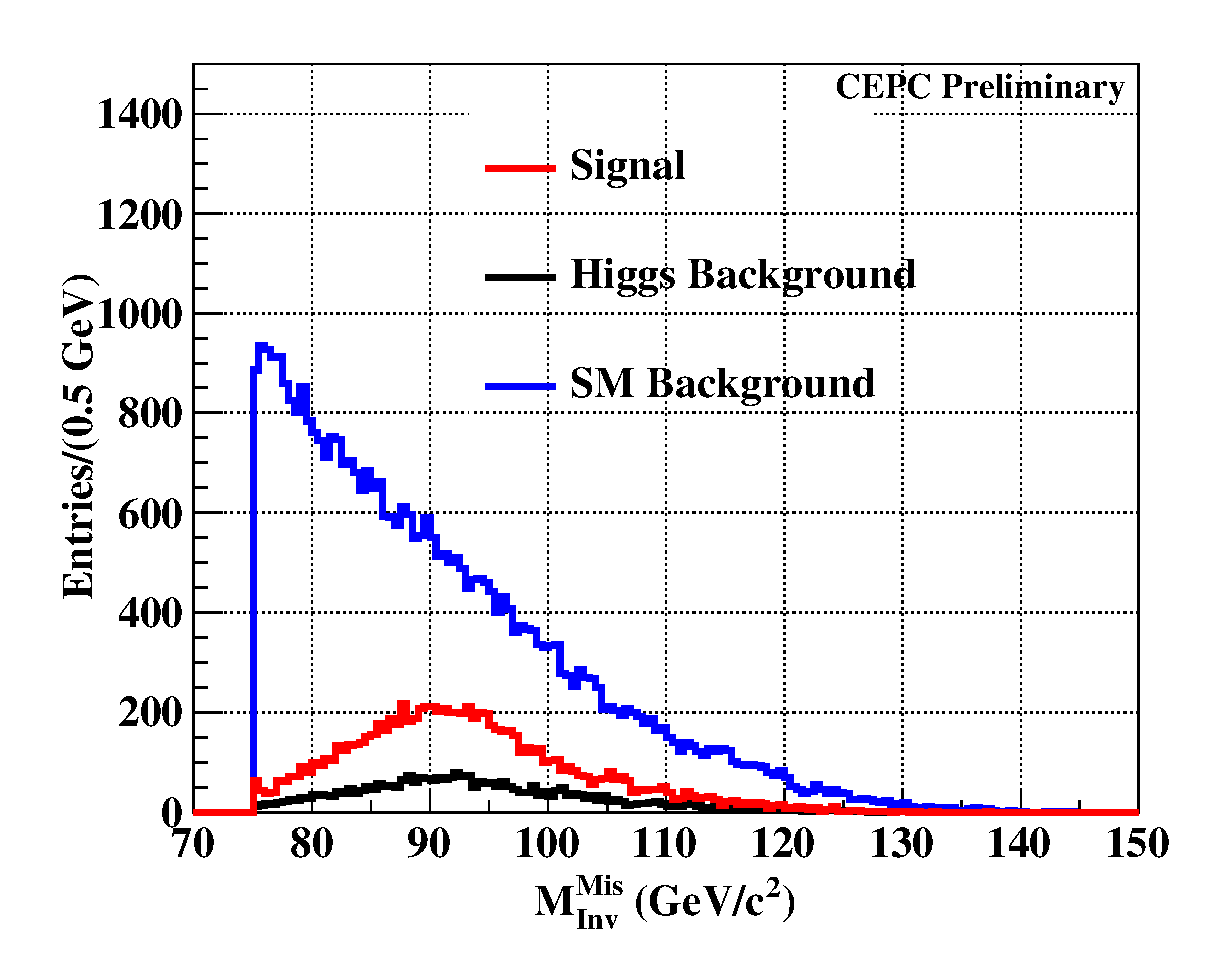
\includegraphics[width=0.5\textwidth]{nnH/fourq/MisMass_AF}
\label{fig:eehuvqqrecfit}
\caption[]{The distribution of recoil mass of $\mu^+\mu^-$ after event selection}
\end{figure}

We can get the number of signal events by counting,
\begin{equation*}
N_{sig} = 9022\pm224 ;
\end{equation*}
and $N_{sig}$ is events of signal, the effeciency of selection $\varepsilon = 37.7\%$. Statistical uncertainty is 
\begin{equation*}
Accu.=\frac{\sqrt{S+B}}{S} = 2.5\%.
\end{equation*}

%After these cuts, we reject the most background, in Table~\ref{tab:eeCutchain}.
%\begin{table}[H]
%  \begin{center}
%    \begin{tabular}{cccc}
%      \hline \hline
%      \multicolumn{1}{c}{Category}      & \multicolumn{1}{c}{Signal}&\multicolumn{1}{c}{$ZH$}&\multicolumn{1}{c}{Single $Z$}\\ 
%      \hline
%      Total		       	 									&      91  	& 37825	&  67758\\
%      $N_{ZPole}=2; N_{Isolep}=2; l_1 = e, l_2 = e$	 		&     60    &   149	& 18179\\
%      $80\gev < M_{Inv}^{e^+e^-} < 100\gev$         		&     55    &   122	& 	10795\\
%	  $120\gev < M_{Rec}^{e^+e^-} < 150\gev$        		&     48    &   115	& 	5045\\
%	  $N_{Remain} < 4$										&	  46	&	71	& 	4873\\
%	  $100\gev < M_{Mis}^{2} < 6000\gev$		        	&     42    &   37  & 	1555\\
%	  $Cos\theta_{ee} > -0.2$			        			&     38    &   26	& 	776\\
%	  $P_{T} > 20\gev$										&	  31	&	19	& 	67\\
%	  $Cos\theta_{(ee of Z)} < 0.7$							&     24    &   14  &   36\\
%	  $\sqrt{(\frac{D0}{sigD0})^2+(\frac{Z0}{sigZ0})^2} < 11$&    22    &   1   &   21\\
%	  $M_{Inv}^{ee} < 60\gev$								&     22    &   1   &   14\\
%      \hline \hline
%    \end{tabular}
%   \caption[Monte Carlo purities in the single lepton sample]{Cut chain of $ee ee$ final state}
%  \label{tab:eeCutchain}
% \end{center}
%\end{table}
%
%\subsubsection{Analysis of $WW^*\rightarrow \mu^+\mu^-\nu\bar{\nu}$}
%This subchannel is similar with $e^+e^-\nu\bar{\nu}$ subchannel, so we will ignore the process of analysis.
%Cutchain is in Table~\ref{tab:uucutchain}
%\begin{table}[H]
%  \begin{center}
%    \begin{tabular}{cccc}
%      \hline \hline
%      \multicolumn{1}{c}{Category}      & \multicolumn{1}{c}{Signal}&\multicolumn{1}{c}{$ZH$}&\multicolumn{1}{c}{Single $Z$}\\ 
%      \hline
%      Total		       	 									& 82	& 37825	& 67758\\
%      $N_{ZPole}=2; N_{Isolep}=2; l_1 = \mu, l_2 = \mu$	 	& 63	& 175	& 4674\\
%      $80\gev < M_{Inv}^{e^+e^-} < 100\gev$         		& 53	& 129	& 2340\\
%	  $120\gev < M_{Rec}^{e^+e^-} < 150\gev$        		& 51	& 121	& 748\\
%	  $N_{Remain} < 5$										& 51	& 71	& 729\\
%	  $0\gev < M_{Mis}^{2} < 6000\gev$			        	& 50	& 41	& 471\\
%	  $\sqrt{(\frac{D0}{sigD0})^2+(\frac{Z0}{sigZ0})^2} < 5$& 50	& 19	& 441\\
%	  $10\gev < M_{Inv}^{ee} < 60\gev$						& 49	& 6		& 115\\
%	  $P_{T} > 10\gev$										& 48	& 6		& 45\\
%	  $Cos\theta_{(ee of Z)} < 0.9$							& 44	& 2		&  26\\
%      \hline \hline
%    \end{tabular}
%   \caption[Monte Carlo purities in the single lepton sample]{Cut chain of $ee \mu\mu$ final state}
%  \label{tab:uucutchain}
% \end{center}
%\end{table}
%
%\subsubsection{Analysis of $WW^*\rightarrow e\mu\nu\bar{\nu}$}
%It's a special subchannel with different lepton flavor. 
%Background will be rejected by different flavor effectively.
%Because of this, the cuts we used are less than the other two subchannel.
%The cutchain is Table~\ref{tab:eucutchain}
%\begin{table}[H]
%  \begin{center}
%    \begin{tabular}{cccc}
%      \hline \hline
%      \multicolumn{1}{c}{Category}      & \multicolumn{1}{c}{Signal}&\multicolumn{1}{c}{$ZH$}&\multicolumn{1}{c}{Single $Z$}\\ 
%      \hline
%      Total		       	 									&  178	& 37825	& 67758\\
%      $N_{ZPole}=2; N_{Isolep}=2; l_1 = e, l_2 = \mu$	 	&  124	& 197	& 1069\\
%      $80\gev < M_{Inv}^{e^+e^-} < 100\gev$         		&  106	& 147	& 585\\
%	  $120\gev < M_{Rec}^{e^+e^-} < 150\gev$        		&  98 	& 139	& 188\\
%	  $N_{Remain} < 4$										&  97	& 106	& 172\\
%	  $0\gev < M_{Mis}^{2} < 5500\gev$		        		&  93 	& 49 	& 72\\
%	  $\sqrt{(\frac{D0}{sigD0})^2+(\frac{Z0}{sigZ0})^2} < 5$&  81 	& 8		& 8\\
%      \hline \hline
%    \end{tabular}
%   \caption[Monte Carlo purities in the single lepton sample]{Cut chain of $ee e\mu$ final state}
%  \label{tab:eucutchain}
% \end{center}
%\end{table}
%
%\subsection{Semi-leptonic decay channel}
%
%The cut chain is here, Table~\ref{tab:semiuvqq}
%\begin{table}[H]
%  \begin{center}
%    \begin{tabular}{ccccc}
%      \hline \hline
%      \multicolumn{1}{c}{Category}      & \multicolumn{1}{c}{Signal}&\multicolumn{1}{c}{$ZH$}&\multicolumn{1}{c}{$ZZ$}&\multicolumn{1}{c}{Single $Z$}\\ 
%      \hline
%      Total 	      	 									&   1221	& 35773	&	109	& 66150\\
%      $N_{ZPole}=2; N_{Isolep}=1; N_{Jets} =2; l = \mu$		&   1048	& 1195	&	33	& 10065\\
%      $80\gev/c^2 < M_{Inv}^{e^+e^-} < 100\gev/c^2$    		&   782		& 1447	&	10	& 4901\\
%	  $120\gev/c^2 < M_{Rec}^{e^+e^-} < 150\gev/c^2$   		&   751 	& 1394	&	6	& 1331\\
%	  $7 < N_{Remain} < 30$									&	722		& 705	& 	1	& 328\\
%	  $15\gev/c^2 < M_{Rec}^{di-Jet} < 95\gev/c^2 $			&	693		& 274	&	1	& 200\\
%	  $Btag < 1$											&	689		& 147	& 	1	& 81\\
%	  $M_{Missing}^2 < 3000\gev^2/c^4$						&   686		& 104	&	1	& 68\\
%	  $\sqrt{(\frac{D0}{sigD0})^2+(\frac{Z0}{sigZ0})^2} < 5$&	684  	&  28 	&	1	& 20\\
%      \hline \hline
%    \end{tabular}
%  \caption[Monte Carlo purities in the single lepton sample]{% Monte
%    Cut chain of semi leptonic decay of $H\rightarrow WW^* \rightarrow \mu\nu qq$}
%  \label{tab:semiuvqq}
%  \end{center}
%\end{table}
%
%\subsubsection{Analysis of $WW^*\rightarrow e\nu qq$}
%Compared to $\mu\nu qq$ subchannel, the resolution of energy and impact parameter of this subchannel are worse,
%and we consider another cut, Figure~\ref{fig:semideltaE}.
%\begin{figure}[H]
%\centering
%\includegraphics[width =0.5\textwidth]{eeh_deltaE_e}
%\caption[]{The distribution of delta energy of di-jet}
%\label{fig:semideltaE}
%\end{figure}
%
%The cut chain is Table~\ref{tab:semievqq}
%\begin{table}[H]
%  \begin{center}
%    \begin{tabular}{ccccc}
%      \hline \hline
%      \multicolumn{1}{c}{Category}      & \multicolumn{1}{c}{Signal}&\multicolumn{1}{c}{$ZH$}&\multicolumn{1}{c}{$ZZ$}&\multicolumn{1}{c}{Single $Z$}\\ 
%      \hline
%      Total 	      	 									&   1182	& 35773	&	109	& 66150\\
%      $N_{ZPole}=2; N_{Isolep}=1; N_{Jets} =2; l = e$		&   916		& 1450	&	11	& 7965\\
%      $80\gev/c^2 < M_{Inv}^{e^+e^-} < 100\gev/c^2$    		&   728		& 947	&	4	& 4032\\
%	  $120\gev/c^2 < M_{Rec}^{e^+e^-} < 150\gev/c^2$   		&   687 	& 879	&	2	& 1386\\
%	  $7 < N_{Remain} < 30$									&	657		& 350	& 	1	& 374\\
%	  $10\gev/c^2 < M_{Rec}^{di-Jet} < 85\gev/c^2 $			&	630		& 184	&	1	& 274\\
%	  $Btag < 1$											&	628		& 132	& 	1	& 142\\
%	  $M_{Missing}^2 < 4000\gev^2/c^4$						&   626		& 101	&	1	& 137\\
%	  $\sqrt{(\frac{D0}{sigD0})^2+(\frac{Z0}{sigZ0})^2} < 40$&  617   	&  85 	&	1	& 130\\
%	  $|\delta E_{Jets}| <60\gev$							&	612		&  75	&	1	& 112\\
%      \hline \hline
%    \end{tabular}
%  \caption[Monte Carlo purities in the single lepton sample]{% Monte
%    Cut chain of semi leptonic decay of $H\rightarrow WW^* \rightarrow e\nu qq$}
%  \label{tab:semievqq}
%  \end{center}
%\end{table}

%
%%%%%%%%%%%%%%%%%%%%%%%%%%%%%%%%%%%%%%%%%%%%%%%%%%%%%%%%%%%%%%%%%%%%%%%%%%%%%%%
% Data characteristics
%%%%%%%%%%%%%%%%%%%%%%%%%%%%%%%%%%%%%%%%%%%%%%%%%%%%%%%%%%%%%%%%%%%%%%%%%%%%%%%
%
%\section{Data characteristics}



%
%%%%%%%%%%%%%%%%%%%%%%%%%%%%%%%%%%%%%%%%%%%%%%%%%%%%%%%%%%%%%%%%%%%%%%%%%%%%%%%
% Systematic uncertainties
%%%%%%%%%%%%%%%%%%%%%%%%%%%%%%%%%%%%%%%%%%%%%%%%%%%%%%%%%%%%%%%%%%%%%%%%%%%%%%%
%
%\section{Systematic uncertainties}

%Give a detailed list of systematic uncertainties, the method
%by which they were obtained, and a justification of the resulting
%values.
%%
%Use ``systematic uncertainty'' instead of ``systematic errors''.
%The latter sounds as if you have made a mistake systematically.

%
%%%%%%%%%%%%%%%%%%%%%%%%%%%%%%%%%%%%%%%%%%%%%%%%%%%%%%%%%%%%%%%%%%%%%%%%%%%%%%%
% Results
%%%%%%%%%%%%%%%%%%%%%%%%%%%%%%%%%%%%%%%%%%%%%%%%%%%%%%%%%%%%%%%%%%%%%%%%%%%%%%%
%
\section{Results}
%\subsection{Statistical uncertainty}
The function of measurement of branch ratio of $H\rightarrow WW^*$ is 
\begin{equation*}
Br(H\rightarrow WW^*) = \frac{N_{sig}}{N_{total} \cdot Br_{rel.} \cdot \varepsilon}
\end{equation*}
$N_{total}=\mathcal{L}\times\sigma_{ZH}$ means total number of events of $ZH$ process; $Br_{rel.}$ means relative branch ratio for 
$Br(H\rightarrow WW^*)$ measurement, including branch fraction of $Z$ boson and $W$ boson; $\varepsilon$ means the efficiency of 
event selection of signal; $N_{sig}$ means the events of signal after event selection.

\begin{table}[H]
  \begin{center}
    \begin{tabular}{cr@{$\pm$}lcc}
      \hline \hline
      Category      &\multicolumn{2}{c}{Signal}& \multicolumn{1}{c}{Relative uncertainty} & \multicolumn{1}{c}{Efficiency of selection}\\ 
      \hline
      $Z\rightarrow e^+e^-; H\rightarrow WW^*\rightarrow e\nu e\nu			$	&20    &7	&35\%   &25.0\%\\
      $Z\rightarrow e^+e^-; H\rightarrow WW^*\rightarrow \mu\nu\mu\nu		$	&44    &8	&18.2\%	&43.1\%\\ 
      $Z\rightarrow e^+e^-; H\rightarrow WW^*\rightarrow e\nu\mu\nu			$	&53    &8	&15.1\% &27.6\%\\
	  $Z\rightarrow e^+e^-; H\rightarrow WW^*\rightarrow e\nu qq			$	&435   &23  &5.3\%  &37.0\%\\
	  $Z\rightarrow e^+e^-; H\rightarrow WW^*\rightarrow \mu\nu qq			$	&551   &24	&4.5\%  &48.0\%\\
      $Z\rightarrow \mu^+\mu^-; H\rightarrow WW^*\rightarrow e\nu e\nu		$	&23    &5	&21.7\% &25.8\%\\
      $Z\rightarrow \mu^+\mu^-; H\rightarrow WW^*\rightarrow \mu\nu\mu\nu	$	&39    &7	&18\%	&44.8\%\\ 
      $Z\rightarrow \mu^+\mu^-; H\rightarrow WW^*\rightarrow e\nu\mu\nu		$	&93    &10	&11\%   &54.1\%\\
	  $Z\rightarrow \mu^+\mu^-; H\rightarrow WW^*\rightarrow e\nu qq		$	&573   &25  &4.0\%  &51.7\%\\
	  $Z\rightarrow \mu^+\mu^-; H\rightarrow WW^*\rightarrow \mu\nu qq		$	&756   &30	&4.4\%  &68.4\%\\
	  $Z\rightarrow \nu\bar{\nu}; H\rightarrow WW^*\rightarrow qqqq			$	&9022  &224	&2.5\%  &37.7\%\\
      \hline \hline
    \end{tabular}
  \caption{Statistic uncertainty of Signal and Relative uncertainty}
  \label{tab:fullstatistic}
  \end{center}
\end{table}
\begin{table}[H]
\begin{center}
\begin{tabular}{cccccc}
\hline\hline
			&	Total events $N$ &	$Br(W\rightarrow l\nu)$  &  $W\rightarrow qq$  &  $Z\rightarrow l^+\l^-$  &  $Z\rightarrow qq$  \\
\hline
Mean value	&	1060000			 &  10.86\%					 &  67.41\%			   &  3.3658\%				  &  69.91\%			\\
Uncertainty	&	$\pm4000$		 &	$\pm0.09\%$				 &  $\pm0.27\%$		   &  $\pm0.0023\%$			  &  $\pm0.06\%$			\\
\hline\hline
\end{tabular}
\caption[]{Relative data for measurement of branch ratio}
\label{tab:relativeresult}
\end{center}
\end{table}

After analysis, the relative uncertainty of signal of 11 subchannels is given in Table~\ref{tab:fullstatistic}, 
and the result of each branch ratio is given by other collabration in Table~\ref{tab:relativeresult}. 
The relative uncertainties of $Z\rightarrow X$, $W\rightarrow X$ and $N_{Total}$ are negligible. 
Relative statistical uncertainty $\Delta{Br(H\rightarrow WW^*)}/Br(H\rightarrow WW^*)$ is 1.62\%.

%\subsection{Systematic uncertainty}
%Because the data we have used are MC data, the analysis of systematic uncertainty should be based on a experienced discussion. 
%And we can refer to the result of LEP due to it is also a electron positron collider.
%\begin{itemize}
%\item Tracker reconstruction: Especially for reconstruction of lepton, it is a main resource of systematic uncertainty. 
%Improving the efficiency of reconstruction would reduce the uncertainty, and we should do research systematically in the future.
%\item Jet clustering: It would be a main influence for measurement of mass of $W$ boson. Energy resolution of jet and flavor tag 
%are two parts of this systematic uncertainty.
%\item MC simulation: In true practice, MC would not match the data totally, so we should reduce the bias between MC and data to 
%decrease this systematic uncertainty when we have true data sample.
%\item Measurement of luminosity: The luminosity of CEPC is given by measurement of BaBar scatter. This measurement would 
%has its own uncertainty, so it is also a resource of systematic uncertainty.
%\end{itemize}
%

%\subsection{Measurement of Higgs width}
%As mentioned before, $\Gamma_H = \frac{Y_1^2 Y_3 F_2 F_4}{F_1^2 F_3 Y_2 Y_4} = f_a\times\frac{\sigma_{\nu\bar{\nu}H}}{Br(H\rightarrow WW^*)}$, 
%and $f_a= \frac{F_2 F_4}{F_1^2 F_3}$ could be caculated in theory. 
%
%%%%%%%%%%%%%%%%%%%%%%%%%%%%%%%%%%%%%%%%%%%%%%%%%%%%%%%%%%%%%%%%%%%%%%%%%%%%%%%
% Discussion
%%%%%%%%%%%%%%%%%%%%%%%%%%%%%%%%%%%%%%%%%%%%%%%%%%%%%%%%%%%%%%%%%%%%%%%%%%%%%%%
%
%\section{Discussion}
%
%Put the results into the context of the theory or a model.
%%
%If the results lead to exclusion plots, make sure that it is clear 
%which region on the plot is excluded.

%
%%%%%%%%%%%%%%%%%%%%%%%%%%%%%%%%%%%%%%%%%%%%%%%%%%%%%%%%%%%%%%%%%%%%%%%%%%%%%%%
% Summary and conclusion
%%%%%%%%%%%%%%%%%%%%%%%%%%%%%%%%%%%%%%%%%%%%%%%%%%%%%%%%%%%%%%%%%%%%%%%%%%%%%%%
%
\section{Summary and conclusion}
11 subchannel of $H\rightarrow WW^*$ process have been analyzed at CEPC. The integrated luminosity of 5000fb$^-1$ and the mass 
of Higgs boson of 125$\gev$ are assumed. The obtained result of accuracy for branch ratio is 1.62\%.

Recently, only about 15\% data has been analyzed. With the CEPC R\&D goes by, the result of analysis would be optimized continuously. 
In the future, $Z\rightarrow qq, H\rightarrow WW^*\rightarrow qqqq$ channel would be analyszed, which would improve the accuracy effectively 
for measurement of branch ratio. Furthermore, CEPC is also a $Z$ boson factory, and it would give us a great support. 
On the one hand, the precision of measurement result about $Z$ boson would be improved, and it would be helpful for precise 
measurement at CEPC. On the other hand, a huge sample would be producted at $Z$ pole, and it would help us to study the 
performance of detector better and reduce the systematic uncertainty.

Later on, there are three parts to be considered. At first, systematic uncertainty has not be discussed. 
And we would do it in the future. Secondly, the isolated lepton finder algorithm is not a general algorithm, and needs to be optimized and 
improved, but it is suitable for recent research. At last, events of signal are got by counting, and we should learn the distribution of 
signal and background deeper and do a fit to improve precision of analysis.
%
%%%%%%%%%%%%%%%%%%%%%%%%%%%%%%%%%%%%%%%%%%%%%%%%%%%%%%%%%%%%%%%%%%%%%%%%%%%%%%%
% Acknowledgements
%%%%%%%%%%%%%%%%%%%%%%%%%%%%%%%%%%%%%%%%%%%%%%%%%%%%%%%%%%%%%%%%%%%%%%%%%%%%%%%

\section{Acknowledgements}

%A standard template for the acknowledgements is available on the
%web pages of the Publication Committee.
Thanks Dr. LI Gang and Dr. RUAN Manqi greatly for their guidance and their constructive arguements.
And thanks my colleagues, Mr. CHEN Zhenxing and Mr. WEI Yuqian who build a good basement for me, 
Dr. MA Bingsong and Dr. MO Xin who are engaged in generator, simulation and reconstruction of samples, 
Dr. WANG Feng who help me solve some technical problems.
%See reference~\cite{publication_policy} for the URL. 

%
%%%%%%%%%%%%%%%%%%%%%%%%%%%%%%%%%%%%%%%%%%%%%%%%%%%%%%%%%%%%%%%%%%%%%%%%%%%%%%%
% Rules for referencing
%%%%%%%%%%%%%%%%%%%%%%%%%%%%%%%%%%%%%%%%%%%%%%%%%%%%%%%%%%%%%%%%%%%%%%%%%%%%%%%
%
%\section{Rules for referencing}
%
%Use \BibTeX{} for the references. See Appendix~\ref{app:References}
%for an explanation.
%
%Only cite permanent, publicly available, or CEPC approved references.
%Private references, not available to the general public, should be
%avoided. Caution should be used when referring to CEPC notes.
%Only reference approved notes. Do not reference COM or INT notes,
%as these are not available outside CEPC.
%
%Whenever possible, cite the article's journal rather than its
%preprint number. If desired, the hep-ex number can be given in
%addition. Always double check references when copying them from
%another source.
%
%Referencing styles are journal-dependent. See the CEPC Publication
%Policy document for more information.

%%%%%%%%%%%%%%%%%%%%%%%%%%%%%%%%%%%%%%%%%%%%%%%%%%%%%%%%%%%%%%%%%%%%%%%%%%%%%%%
% Bibliography
%%%%%%%%%%%%%%%%%%%%%%%%%%%%%%%%%%%%%%%%%%%%%%%%%%%%%%%%%%%%%%%%%%%%%%%%%%%%%%

\bibliographystyle{cepcBibStyleWoTitle}
\bibliography{instructions}

%%%%%%%%%%%%%%%%%%%%%%%%%%%%%%%%%%%%%%%%%%%%%%%%%%%%%%%%%%%%%%%%%%%%%%%%%%%%%%%
% Technical Aspects
%%%%%%%%%%%%%%%%%%%%%%%%%%%%%%%%%%%%%%%%%%%%%%%%%%%%%%%%%%%%%%%%%%%%%%%%%%%%%%%

\newpage
\appendix
\part*{Appendices}
\addcontentsline{toc}{part}{Appendices}

%Use the Appendices to include all the technical details of your work
%that are relevant for the CEPC Collaboration only (e.g. datases
%details, software release used). The Appendices can be removed from
%an CEPC Internal Note becoming an CEPC Public Note.
%
%Use the following commands to start the Appendices section:
%\begin{verbatim}
%   \newpage
%   \appendix
%   \part*{Appendices}
%   \addcontentsline{toc}{part}{Appendices}
%\end{verbatim}

\section{Isolated leptons' condition}
\label{app:isolepcondition}
Isolated leptons tagging is a key in $WW^*$ analysis, espcially in jets environment, so a good iaolated leptons algorithm
could decide our analysis accuracy. We will introduce the isolated leptons algorithm below:\\
There are two key conditions. The first one is lepton identification that a good PFA could help us.
The second is isolated conditions, cone angle of lepton and the ratio of energy in cone angle and lepton's energy, 
shown in Table~\ref{tab:isolep}.
\begin{table}[H]
\begin{center}
\begin{tabular}{cccccc}
\hline \hline
\multirow{2}{*}{$E_{lepton}$} & \multirow{2}{*}{Leptons' flavor} 	& \multicolumn{2}{c}{Full-leptonic Decay} 
& \multicolumn{2}{c}{Semi-leptonic Decay}\\
							&									&Cone Angle[rad]&$E_{Cone}/E_{Lepton}$
							&Cone Angle[rad]&$E_{Cone}/E_{Lepton}$\\
\hline
\multirow{2}{*}{$5\gev-10\gev$}	&			Muon					&0.15		&0.25		&0.15		&0.7	\\
							&			Electron				&0.3		&1.1		&0.3		&0.9	\\
\hline
\multirow{2}{*}{$10\gev-15\gev$}	&			Muon					&0.15		&0.35		&0.15		&0.25	\\
							&			Electron				&0.3		&0.75		&0.3		&0.75	\\
\hline
\multirow{2}{*}{$>15\gev$}	&			Muon					&0.15		&0.3		&0.15		&0.25	\\
							&			Electron				&0.25		&0.55		&0.25		&0.6	\\
\hline \hline
\end{tabular}
\caption{Isolated lepton condition}
\label{tab:isolep}
\end{center}
\end{table}
%\section{The {\tt cepcnote} class}
%\label{app:CepcNoteCls}
%
%This paper has been typeset using the {\tt cepcnote.cls} class, that
%implement the CEPC template can be used for papers, preprints,
%notes. The {\tt cepcnote} class is available on web pages of the
%Publication Committee, as well as this instruction paper and the
%related files.
%
%{\tt cepcnote.cls} derives from the standard \LaTeX{} {article.cls}
%class, thus all the usual commands and options you would have used
%with {\tt article} will work with it. For instance, this paper has
%been produced using this very simple preamble:
%
%\begin{verbatim}
%  \documentclass[11pt,a4paper]{cepcnote}
%  \graphicspath{{figures/}}
%  \usepackage{cepcphysics}
%  \usepackage{subfigure}
%\end{verbatim}
%
%\subsection{Dependencies}
%
%The {\tt cepcnote} class depends on these packages, which presence in
%your system is required:
%\begin{itemize}
%  \item {\tt graphicx}
%  \item {\tt mathptmx}
%  \item {\tt lineno}
%\end{itemize}
%The first two are all usually already installed in any modern \LaTeX{}
%installation, while the latter is part of the {\tt ednotes} package
%bundle and is direclty provided with this package; {\tt cepcnote} was
%tested on a IHEP {\tt lxslc} login node and worked out of the box. The {\tt
%  cepcnote} class works both with \LaTeX{} and pdf\LaTeX{}.
%
%If you wish to use the {\tt cepccover} package with the {\tt
%  cepcnote} class, load the latest version of the package in your
%system, and invoke it using the {\tt coverpage} option of the class:
%\begin{verbatim}
%  \documentclass[11pt,a4paper,coverpage]{cepcnote}
%\end{verbatim}
%instead of the the usual {\tt usepackage} command: this will ensure
%that the cover page is produced before the note title page.
%
%\subsection{Custom commands}
%
%The {\tt cepcnote} class implements some custom commands, mainly
%used to typeset the frontpage content:
%
%\begin{itemize}
%
%  \item {\verb|\title{<Title>}|} typesets the paper title. If not
%    given, a dummy \emph{Title goes here} title will be produced.
%
%  \item {\verb|\author{<Author>}|} typesets the paper author. If not
%    explicitly given, \emph{The CEPC Collaborations} will be used by
%    default. Note that the \verb|\author{}| command is pretty limited
%    in case you want to display multiple author names and multiple
%    affiliations. For this use case the \verb|authblk.sty| package is
%    provided; this is a typical example of its use:
%    \begin{verbatim}
%\usepackage{authblk}
%\renewcommand\Authands{, } % avoid ``. and'' for last author
%\renewcommand\Affilfont{\itshape\small} % affiliation formatting
%
%\author[a]{First Author}
%\author[a]{Second Author}
%\author[b]{Third Author}
%
%\affil[a]{One Institution}
%\affil[b]{Another Institution}
%    \end{verbatim}
%  \item {\verb|\mail{<Mail address>}|} typesets only one E-mail address in the foot note.
%
%  \item {\verb|\abstracttext{<The abstract text>}|} typesets the
%    abstract in the front page.
%
%  \item {\verb|\date{<Date>}|} typesets the paper date. If not
%    explicitly given, the current date (\verb|\today|) will be used.
%
%  \item {\verb|\draftversion{<Draft Version>}|} displays the draft
%    version on the front page, a DRAFT banner on all the other page
%    headings, and add line numbers to all text to easy commenting abd
%    reviewing. Can be omitted.
%
%  \item {\verb|\journal{<Journal Name>}|} displays the phrase \emph{to
%    be submitted to Journal Name} at the bottom of the front page. Can
%    be omitted.
%
%  \item {\verb|\skipbeforetitle{<lenght>}|} sets the distance between
%    the title page header and the note title. The default value should
%    be fine for most notes, but in case you have a long list of
%    authors or a lenghtly abstract you can use this command to buy
%    some extra space. Note that \verb|<lenght>| can also be negative
%    (use it at your own risk!).
%
%\end{itemize}
%
%\noindent {\tt emptynote.tex} contains a basic skeleton that can be
%used to start typing a new note using the {\tt cepcnote} class. All
%the custom commands described above are used in this example file, in
%order to demonstrate their use.

%\section{Bibliography}
%\label{app:References}

%We recommend to use \BibTeX{} for the references. Although it often
%appears harder to use at the beginning, it means that the number of
%typos should be reduced significantly and the format of the references
%will be correct, without you having to worry about formatting it. In
%addition the order of the references is automatically correct.
%
%A file with the extension {\tt .bib} (in this example: {\tt
%instruction.bib}) should contain all the references. This file may
%also contain references that you do not use, so it may act like a
%library of references. The typical compilation cycle when using
%\BibTeX{} looks like the following:
%%
%\begin{verbatim}
%  (pdf)latex instructions
%  bibtex instructions
%  (pdf)latex instructions
%  (pdf)latex instructions
%\end{verbatim}
%%
%\BibTeX{} will create a file with the extension {\tt .bbl}, which will
%contain the actual references used, and \LaTeX{} will then take care
%to include them in your paper. Note that only after the third run of
%\LaTeX{} will all references be correct. Unless you change a reference
%you do not have to do the {\tt bibtex} step again.
%
%A \BibTeX{} style file ({\tt cepcBibStyleWoTitle.bst}) is provided with the
%CEPC template. You can use it in your text source file like in the
%following:
%%
%\begin{verbatim}
%  \bibliographystyle{cepcBibStyleWoTitle}
%  \bibliography{instructions}
%\end{verbatim}
%%
%
%{\color{red} \textbf{Important}:} for further information on \BibTeX{} and on the standard CEPC style for referencing, look at the ``{\tt QuickGuide\_BIBTEX}" file shipped with this package.
%
%
%\section{Miscellaneous \LaTeX{} tips}
%\label{app:LatexTips}
%
%\subsection{Graphics}
%
%Use the {\tt graphicx} package \cite{} to include your plots and
%figure. The use of older packages like {\tt espfig} is deprecated.
%Since the {\tt graphicx} package is required by the {\tt cepcnote}
%class, it is automatically loaded when using it, and there is no need
%to explicitly included it in the document preamble.
%
%Always include your graphics file without metioning the file
%extension. Fior inctance, if you want to include the {\tt figure.eps}
%file, you should use a sysntax like this:
%\begin{verbatim}
%  \includegraphics[width=\textwidth]{figure}
%\end{verbatim}
%This will allow to compile your document using either \LaTeX{} or
%pdf\LaTeX{} without changing your source file: you can in fact have
%both {\tt figure.eps} and {\tt figure.pdf} in your working directorym
%and the proper one will be picked up according to the processing method
%you chose.
%
%It is a good habit to keep you graphics file in a separated
%sub-directory (e.g. in {\tt figure/}. In this case you can include them
%by mentioning it explicitly every time:
%\begin{verbatim}
%  \includegraphics[width=\textwidth]{figures/figure}
%\end{verbatim}
%or by telling once for all to the {\tt graphicx} package where to look
%for them, by using this command:
%\begin{verbatim}
%  \graphicspath{{figures/}}
%\end{verbatim}
%
%
%\subsection{Definitions}
%
%You can use \verb|\ensuremath| in definitions, so that they will work
%in both text mode and math mode, e.g.
%\verb|\newcommand{\UoneS}{\ensuremath{\Upsilon(\mathrm{1S})}}| to get
%\UoneS{} in either mode (\verb|\UoneS{}| or \verb|$\UoneS$|).
%
%\subsection{Emphasis}
%
%Use italics for emphasis sparingly: too many italicized words defeat
%their purpose. When you do italicize a word, really italicize it: do
%not use math mode! Note the difference between \emph{per se}
%(\verb|\emph{per se}|) and $per se$ (\verb+$per se$+). Abbreviations
%like i.e., e.g., etc., and et al. should \emph{not} be italicized!
%For program names we recommend to use small capitals:
%\verb|{\sc Pythia}}| produces {\sc Pythia}.
%
%\section{General Style}
%
%We recommend the use of British English. However, whatever you decide
%to choose, be consistent throughout the paper. For much more detailed
%information on writing, spelling and typographic style, etc. please
%see the CEPC Style Guide \cite{}. The CEPC Publication Policy
%contains a list of CEPC detector acronyms. Standard ways to write
%these are in the CEPC Glossary.
%
%\section{The {\tt cepcphysics.sty} style file}
%\label{app:CepcPhysicsSty}
%
%The {\tt cepcphysics.sty} style file implements a series of useful
%shortcut to typeset a physics paper, such as units or particle
%symbols. It can included in the preamble of your paper with the usual
%syntax:
%
%\begin{verbatim}
%  \usepackage{cepcphysics}
%\end{verbatim}
%
%\subsection{Remarks on units and symbols}
%
%Use SI units in roman-type font. Leave a \emph{small} space between
%the value and the units (e.g. 12\,mm), and make sure they end up
%always together on the same line. \verb|12\,mm| will fulfill both the
%requirements. Natural units, where $c=\hbar=1$, should be used for all
%CEPC publications. Masses are therefore in \GeV, not \GeV/$c^2$.
%
%Use the shortcut \verb|\GeV{}| (\GeV{}) defined by {\tt
%cepcphysics.sty} instead of just typing \verb|GeV| (GeV), in order
%not to leave a large space between the \emph{e} and the
%\emph{V}. Symbols \verb|\TeV|, \verb|\MeV|, \verb|\keV| and \verb|\eV|
%also exist. In math mode the symbol leaves a space between the number
%and the unit, i.e. the beam energy is \verb+$7\TeV$+ ($7\TeV$). The
%symbol works in text mode and in math mode i.e. \verb+99.0 \MeV+
%(99.0 \MeV), \verb+$88.4\keV$+ ($88.4\keV$).
%
%Use math mode for all symbols (e.g. use $c$ (\verb|$c$|) rather than
%simply c). Momentum is a lower case \verb+$p$+. Transverse momentum is
%a lower case $p$ with an upper case $T$ subscript: \verb|\pT| produces
%\pT. Energy is an upper case \verb+$E$+, \verb+\ET+ produces \ET.  Use
%\verb|\mathscr| mode for luminosity $\mathscr{L}$ or aplanarity
%$\mathscr{A}$, including the package \verb|mathrsfs.sty|.
%
%Trigonometric functions should be in roman type. Natural logarithm
%should be ln and log base 10 is log.  When in math mode, use
%\verb+$\ln$, $\sin$,+ etc. We recommend to specify the base of the
%logarithm: \verb+$\log_{10}$+.
%
%If your note makes use of cones, for example cone-jets, explain that
%these cones are constructed in $\eta$-$\phi$ space, and define $\eta$.
%
%Add the word \emph{events} as the unit when quoting the number of
%events: ``The resulting background is $4.0 \pm 1.3$ events.''.  The
%number of expected events should be written as $N_{\rm pred}$ rather
%than $N_{\rm exp}$, since the latter could also mean experimental.
%
%For particle names and symbols, CEPC uses the standards of the
%Particle Data Book. Intermediate vector bosons should be called
%\emph{W boson(s)} and \emph{Z boson(s)}, not just \emph{W's} or
%\emph{Ws}. The Z boson should not have a superscript of 0. W without
%the word boson attached may be used in \emph{W pair production}, and
%similar phrases.  Other particle names should be spelled out when used
%in a sentence: muon(s), electron(s), tau lepton(s). \emph{Top quark}
%should be used instead of \emph{top} in most places: say ``top quark
%mass'' instead of ``top mass''.  Top quark and bottom quark may be
%shortened to \emph{$t$ quark} and \emph{$b$ quark}. The neutrino
%symbol $\nu$ should not have any subscripts, unless necessary for
%understanding. For the \Jpsi{} use the command \verb+\Jpsi+ from {\tt
%cepcphysics.sty}: it will produce a lower case $\psi$.
%
%When in doubt, use the PDG style.
%
%\subsection{Other shortcuts}
%
%\noindent The {\tt cepcphysics.sty} style file contains among
%other things:
%
%\medskip
%
%\begin{tabular}{llcllcll}
%  \verb+\lapprox+ & \lapprox{} & \hspace{1cm} &
%  \verb+\rapprox+ & \rapprox{}  &\hspace{1cm} &
%  \verb+\rts+  & \rts{} \\
%  \verb+\Ecm+ & \Ecm{} & &
%  \verb+\stat+ & \stat{} & &
%  \verb+\syst+ & \syst{} \\
%\end{tabular}
%
%\medskip
%
%\begin{tabular}{llcllcll}
%  \verb+\Zboson+ & \Zboson{} & \hspace{5mm} &
%  \verb+\Wboson+ & \Wboson{} & \hspace{5mm} &
%  \verb+\Wplus+ & \Wplus{} \\
%  \verb+\Wminus+ & \Wminus{} & &
%  \verb+\Wpm+ & \Wpm{} & &
%  \verb+\Wmp+ & \Wmp{} \\
%  \verb+\Afb+ & \Afb{} & &
%  \verb+\GW+ & \GW{} & &
%  \verb+\GZ+ & \GZ{} \\
%  \verb+\Wln+ & \Wln{} & &
%  \verb+\Zll+ & \Zll{} & &
%  \verb+\Zee+ & \Zee{} \\
%  \verb+\Zmm+ & \Zmm{} & &
%  \verb+\mZ+ & \mZ{} \\
%  \verb+\mW+ & \mW{} & &
%  \verb+\mH+ & \mH{} \\
%  \verb+\Mtau+ & \Mtau{} & &
%  \verb+\swsq+ & \swsq{} & &
%  \verb+\swel+ & \swel{} \\
%  \verb+\swsqb+ &  \swsqb{} & &
%  \verb+\swsqon+ & \swsqon{} & &
%  \verb+\gv+ &  \gv{} \\
%  \verb+\ga+ & \ga{} & &
%  \verb+\gvbar+ & \gvbar{} & &
%  \verb+\gabar+ & \gabar{} \\
%  \verb+\Zprime+ & \Zprime{} & &
%  \verb+\Hboson+ & \Hboson{} & & 
%  \verb+\GH+ & \GH{} \\
%\end{tabular}
%
%\medskip
%
%\noindent The command \verb+\Zzero+ is identical to \verb+\Zboson+.
%
%\medskip
%
%\begin{tabular}{llcllcll}
%  \verb+\tbar+ & \tbar{} & \hspace{1cm} &
%  \verb+\ttbar+ & \ttbar{} & \hspace{1cm} &
%  \verb+\bbar+ & \bbar{} \\
%  \verb+\bbbar+ & \bbbar{} & &
%  \verb+\cbar+ & \cbar{} & &
%  \verb+\ccbar+ & \ccbar{} \\
%  \verb+\sbar+ & \sbar{} & &
%  \verb+\ssbar+ &  \ssbar{} & &
%  \verb+\ubar+ & \ubar{} \\
%  \verb+\uubar+ & \uubar{} & &
%  \verb+\dbar+ & \dbar{} & &
%  \verb+\ddbar+ & \ddbar{} \\
%  \verb+\fbar+ & \fbar{} & &
%  \verb+\ffbar+ &  \ffbar{} & &
%  \verb+\qbar+ & \qbar{} \\
%  \verb+\qqbar+ & \qqbar{} & &
%  \verb+\nbar+ & \nbar{} & &
%  \verb+\nnbar+ & \nnbar{} \\
%  % \verb+\e+ & \e{} & &
%  \verb+\ee+ & \ee{} & &
%  \verb+\mumu+ & \mumu{} & &
%  \verb+\tautau+ & \tautau{} \\
%  \verb+\epm+ & \epm{} & &
%  % \verb+\epem+ & \epem{} & &
%  \verb+\leplep+ & \leplep{} & & 
%  \verb+\lnu+ & \lnu{} \\
%  % \verb+\ellell+ & \ellell{} & & & \\
%\end{tabular}
%
%\medskip
%
%\begin{tabular}{llcllcll}
%  \verb+\BoBo+ & \BoBo{} & \hspace{1cm} &
%  \verb+\BodBod+ & \BodBod{} & \hspace{1cm} &
%  \verb+\BosBos+ & \BosBos{} \\
%  \verb+\Bd+ & \Bd{} & &
%  \verb+\Bs+ & \Bs{} & &
%  \verb+\Bu+ & \Bu{} \\
%  \verb+\Bc+ & \Bc{} & &
%  \verb+\Lb+ & \Lb{} & &
%  \verb+\jpsi+ & \jpsi{} \\
%  \verb+\Jpsi+ & \Jpsi{} & &
%  \verb+\Jee+ & \Jee{} & &
%  \verb+\Jmm+ & \Jmm{} \\
%  \verb+\psip+ & \psip{} & &
%  \verb+\kzero+ & \kzero{} & &
%  \verb+\kzerobar+ & \kzerobar{} \\
%  \verb+\kaon+ & \kaon{} & &
%  \verb+\kplus+ & \kplus{} & &
%  \verb+\kminus+ & \kminus{} \\
%  \verb+\klong+ & \klong{} & &
%  \verb+\kshort+ & \kshort{} & &
%  \verb+\Ups+ & \Ups{} \\
%\end{tabular}
%
%\medskip
%
%\begin{tabular}{llcllcllcll}
%  \verb+\alphas+ & \alphas{} & \hspace{1cm} &
%  \verb+\Lms+ & \Lms{} & \hspace{1cm} &
%  \verb+\Lmsfive+ & \Lmsfive{} & \hspace{1cm} &
%  \verb+\KT+ & \KT{} \\
%\end{tabular}
%
%\medskip
%
%\begin{tabular}{llcllcll}
%  \verb+\Vud+ & \Vud{} & \hspace{1cm} &
%  \verb+\Vus+ & \Vus{} & \hspace{1cm} &
%  \verb+\Vub+ & \Vub{} \\
%  \verb+\Vcd+ & \Vcd{} &  &
%  \verb+\Vcs+ & \Vcs{} &  &
%  \verb+\Vcb+ & \Vcb{} \\
%  \verb+\Vtd+ & \Vtd{} & &
%  \verb+\Vts+ & \Vts{} & & 
%  \verb+\Vtb+ & \Vtb{} \\
%\end{tabular}
%
%\medskip
%
%\begin{tabular}{llcllcll}
%  \verb+\Azero+ & \Azero{} & \hspace{1cm} &
%  \verb+\hzero+ & \hzero{} & \hspace{1cm} &
%  \verb+\Hzero+ & \Hzero{} \\
%  \verb+\Hplus+ & \Hplus{} & &
%  \verb+\Hminus+ & \Hminus{} & &
%  \verb+\Hpm+ & \Hpm{} \\
%  % \verb+\Hmp+ \Hmp{}
%\end{tabular}
%
%\medskip
%
%\noindent A generic macro \verb+\susy#1+ is defined, so that for
%example \verb+\susy{q}+ produces \susy{q} and similar.
%
%\medskip
%
%\begin{tabular}{llcllcll}
%  \verb+\chinop+ & \chinop{} & \hspace{1cm} &
%  \verb+\chinotwom+ & \chinotwom{} & \hspace{1cm} &
%  \verb+\chinopm+ & \chinopm{} \\
%  \verb+\nino+ & \nino{} & &
%  \verb+\ninothree+ & \ninothree{} & &
%  \verb+\gravino+ & \gravino{} \\
%  \verb+\squark+ & \squark{} & &
%  \verb+\gluino+ & \gluino{} & &
%  \verb+\slepton+ & \slepton{} \\
%  \verb+\stop+ & \stop{} & &
%  \verb+\stopone+ & \stopone{} & &
%  \verb+\stopL+ & \stopL{} \\
%  \verb+\sbottom+ & \sbottom{} & &
%  \verb+\sbottomtwo+ & \sbottomtwo{} & &
%  \verb+\sbottomR+ & \sbottomR{} \\
%  \verb+\sleptonL+ & \sleptonL{} & &
%  \verb+\sel+ & \sel{} & &
%  \verb+\smuR+ & \smuR{} \\
%  \verb+\stauone+ & \stauone{} & &
%  \verb+\snu+ & \snu{} & &
%  \verb+\squarkR+ & \squarkR{} \\
%\end{tabular}
%
%\medskip
%
%\noindent For \susy{q}, \susy{t}, \susy{b}, \slepton, \sel, \smu and
%\stau, L and R states are defined; for stop, sbottom and stau also the
%light (1) and heavy (2) states. There are four neutralinos and two
%charginos defined, the index number unfortunately needs to be written
%out completely. For the charginos the last letter(s) indicate(s) the
%charge: p for +, m for -, and pm for $\pm$.
%
%\medskip
%
%\begin{tabular}{llcllcll}
%  \verb+\pt+ & \pt{} & \hspace{1cm} &
%  \verb+\pT+ & \pT{} & \hspace{1cm} &
%  \verb+\et+ & \et{} \\
%  \verb+\eT+ & \eT{} & &
%  \verb+\ET+ & \ET{} & &
%  \verb+\HT+ & \HT{} \\
%  \verb+\ptsq+ & \ptsq{} & &
%  \verb+\met{}+ & \met{} & &
%\end{tabular}
%
%\medskip
%
%\noindent Use \verb+\met{}+ rather than just \verb+\met+ to get the spacing
%right. In principle this works for any macro, although in most cases it will
%not be needed as {\tt xspace.sty} will take care of the spacing. Somehow
%{\tt xspace.sty} doesn't do a good job for \met.
%
%\vspace{5mm}
%
%\begin{tabular}{llcllcll}
%\verb+\ifb+ & \ifb{} & \hspace{1cm} &
%\verb+\ipb+ & \ipb{} & \hspace{1cm} &
%\verb+\inb+ & \inb{} \\
%\verb+\TeV+ & \TeV{} & &
%\verb+\GeV+ & \GeV{} & &
%\verb+\MeV+ & \MeV{} \\
%\verb+\keV+ & \keV{} & &
%\verb+\eV+ & \eV{} & & & \\
%\end{tabular}
%
%\medskip
%
%\noindent And \verb+\tev+, \verb+\gev+, \verb+\mev+, \verb+\kev+, and
%\verb+\ev+ have the same results.
%
%\medskip
%
%\noindent A generic macro \verb+\mass#1+ is defined, so that for example
%\verb+\mass{\mu}+ produces \mass{\mu} and similar.
%\verb+\twomass{\mu e}+ will produce \twomass{\mu e}.

\end{document}
